%  BE Mini Project Report - STQA Manual Testing (LP-IV)
%  Manual Testing of an E-Commerce Website Using Test Cases and Bug Reports
%  Based on BE_PROJECT_REPORT_FORMAT_TERM_II_LATEX_FILE.tex (SPPU format)

\documentclass[oneside,a4paper,12pt]{report}

\usepackage{graphicx}
\usepackage{fancyhdr}
\usepackage{titlesec}
\usepackage{listings}
\usepackage{xcolor}
\usepackage{amsmath}
\usepackage[a4paper,margin=1in]{geometry}

\fancypagestyle{plain}{%
  \fancyhf{}
  \fancyfoot[C]{NBN SSOE, Department of Computer Engineering 2026-27}
  \fancyfoot[R]{\thepage}
}
\pagestyle{fancy}
\fancyhead{}
\renewcommand{\headrulewidth}{0pt}
\footskip = 0.625in
\cfoot{}
\rfoot{}

\usepackage[hidelinks]{hyperref}
\usepackage{tikz}
\usetikzlibrary{arrows,shapes,snakes,automata,backgrounds,petri,positioning,calc,fit}

\usepackage{tabularx}
\usepackage[nottoc,notlot,notlof,numbib]{tocbibind}
\usepackage[titletoc]{appendix}
\renewcommand{\appendixname}{Annexure}
\usepackage{titletoc}
\renewcommand{\bibname}{References}
\setcounter{secnumdepth}{5}
\usepackage{float}
\usepackage{subcaption}
\usepackage{multirow}
\usepackage[ruled,vlined]{algorithm2e}

\newcommand{\frontmatter}{\clearpage\pagenumbering{roman}}
\newcommand{\mainmatter}{\clearpage\pagenumbering{arabic}\setcounter{page}{1}}

\lstset{basicstyle=\ttfamily\footnotesize, breaklines=true, frame=single,
  columns=fullflexible, keepspaces=true, showstringspaces=false,
  keywordstyle=\color{blue}, commentstyle=\color{gray}, stringstyle=\color{red!60!black}}

\newcommand{\ptitle}{Manual Testing of an E-Commerce Website Using Test Cases and Bug Reports}
\newcommand{\ptitleshort}{Manual Testing of an E-Commerce Website}

\begin{document}

\setlength{\parindent}{0mm}
\begin{center}

\includegraphics[width=70pt]{sppulogo.jpg}\\
{\bfseries SAVITRIBAI PHULE PUNE UNIVERSITY \\}
 \vspace*{1\baselineskip}
{\bfseries A  MINI PROJECT REPORT ON \\}
 \vspace*{2\baselineskip}
{\bfseries \fontsize{16}{12} \selectfont \ptitle \\ \vspace*{2\baselineskip}}
{\fontsize{12}{12} \selectfont SUBMITTED TOWARDS THE
 \\PARTIAL FULFILLMENT OF THE REQUIREMENTS OF \\
 LABORATORY PRACTICE IV (SOFTWARE TESTING AND QUALITY ASSURANCE)\\
\vspace*{2\baselineskip}}
{\bfseries \fontsize{14}{12} \selectfont BACHELOR OF ENGINEERING (Computer
Engineering) \\
\vspace*{1\baselineskip}}
{\bfseries \fontsize{14}{12} \selectfont BY \\
\vspace*{1\baselineskip}}
Vishwajeet Tulse  \hspace{25 mm} Exam No: \underline{\hspace{25mm}}  \\
Student Name 2 \hspace{25 mm} Exam No: \underline{\hspace{25mm}}   \\
Student Name 3 \hspace{25 mm} Exam No: \underline{\hspace{25mm}}  \\
Student Name 4 \hspace{25 mm} Exam No: \underline{\hspace{25mm}}\\
\vspace*{2\baselineskip}
{\bfseries \fontsize{14}{12} \selectfont Under The Guidance of \\
\vspace*{1\baselineskip}}
Prof. Guide Name\\
\vspace*{1\baselineskip}

\includegraphics[width=100pt]{SinhgadLogo.jpg} \\
{\bfseries \fontsize{14}{12} \selectfont DEPARTMENT OF COMPUTER ENGINEERING \\
NBN SINHGAD SCHOOL OF ENGINEERING \\
10/1, AMBEGAON (BK), PUNE-411041 \\
2026-27
}
\end{center}

\newpage

\begin{figure}[ht]
\centering

\includegraphics[width=100pt]{SinhgadLogo.jpg}
\end{figure}

{\bfseries \fontsize{14}{12} \selectfont \centerline{NBN SINHGAD SCHOOL OF ENGINEERING}
\centerline{DEPARTMENT OF COMPUTER ENGINEERING}
\vspace*{2\baselineskip}}

{\bfseries \fontsize{16}{12} \selectfont \centerline{CERTIFICATE}
\vspace*{2\baselineskip}}

\centerline{This is to certify that the Mini Project Entitled}
\vspace*{.5\baselineskip}

{\bfseries \fontsize{14}{12} \selectfont \centerline{\ptitleshort}
\vspace*{0.5\baselineskip}}

\centerline{Submitted by}
\vspace*{0.5\baselineskip}
\centerline{Vishwajeet Tulse  \hspace{25 mm} Exam No: \underline{\hspace{25mm}} }
\centerline{Student Name 2 \hspace{25 mm} Exam No: \underline{\hspace{25mm}}  }
\centerline{Student Name 3 \hspace{25 mm} Exam No: \underline{\hspace{25mm}} }
\centerline{Student Name 4 \hspace{25 mm} Exam No: \underline{\hspace{25mm}} }
\vspace*{0.5\baselineskip}

is a bonafide work carried out by Students under the supervision of Prof. Guide Name and it
is submitted towards the partial fulfillment of the requirement of Bachelor of Engineering (Computer Engineering) for the course Laboratory Practice IV.\\

\bgroup
\def\arraystretch{0.7}
\vspace*{0.5\baselineskip}
\begin{tabular}{c c }
Prof. Guide Name &  \hspace{50 mm} Dr. S. P. Bendale \\
Internal Guide   &  \hspace{50 mm} H.O.D \\
Dept. of Computer Engg.  &	\hspace{50 mm}Dept. of Computer Engg.  \\
\end{tabular}
\egroup
\vspace*{0.5\baselineskip}
\begin{center}
{
Dr. S. P. Patil \\
Principal\\
NBN Sinhgad School of Engineering
}
\end{center}
\vspace*{1\baselineskip}
Signature of Internal Examiner \hspace{30 mm} Signature of External Examiner
\newpage

\begin{center}
\textbf{PROJECT APPROVAL SHEET}
\end{center}
\begin{center}
 \ptitle
 \end{center}
\begin{center}
Is successfully completed by
\end{center}
\centerline{Vishwajeet Tulse  \hspace{25 mm} Exam No: \underline{\hspace{25mm}} }
\centerline{Student Name 2 \hspace{25 mm} Exam No: \underline{\hspace{25mm}}  }
\centerline{Student Name 3 \hspace{25 mm} Exam No: \underline{\hspace{25mm}} }
\centerline{Student Name 4 \hspace{25 mm} Exam No: \underline{\hspace{25mm}} }
\begin{center}
 at
 \end{center}
 \begin{center}
 DEPARTMENT OF COMPUTER ENGINEERING
 \end{center}
 \begin{center}
 NBN SINHGAD SCHOOL OF ENGINEERING, PUNE
 \end{center}
 \begin{center}
 SAVITRIBAI PHULE PUNE UNIVERSITY, PUNE
 \end{center}
 \begin{center}
 ACADEMIC YEAR 2026-2027
 \end{center}
 \vspace*{1\baselineskip}
 \begin{tabular}{c c }
Prof. Guide Name &  \hspace{50 mm} Dr. S. P. Bendale \\
Internal Guide   &  \hspace{50 mm} H.O.D \\
Dept. of Computer Engg.  &	\hspace{50 mm}Dept. of Computer Engg.  \\
\end{tabular}
\newpage

\setcounter{page}{0}
\frontmatter
\cfoot{NBN SSOE, Department of Computer Engineering 2026-27}
\rfoot{\thepage}
\pagenumbering{Roman}

{  \newpage {\bfseries \fontsize{14}{12} \selectfont \centerline{Abstract}
\vspace*{2\baselineskip}} \setlength{\parindent}{11mm} }
{ \setlength{\parindent}{0mm} }
Manual testing is the foundation of software quality assurance: a tester studies the requirements, designs test cases, executes them by hand in the real application and records what actually happens. This mini project applies the complete manual testing process to \textbf{Swag Labs} (\url{https://www.saucedemo.com}), a publicly available demo e-commerce website that offers login, a product catalogue, a shopping cart and a checkout flow. The site provides six test user accounts, several of which deliberately expose functional, visual and performance defects, which makes it an ideal subject for learning defect detection and reporting.

The work followed the standard test life cycle. A test plan defined the scope, strategy, environment and entry/exit criteria. Twenty test scenarios were derived from the application's features and expanded into thirty-nine test cases written in an Excel sheet with pre-conditions, steps, test data, expected and actual results, status and priority. Black-box techniques (equivalence partitioning, boundary values, error guessing) were used to design positive and negative cases, in particular for the login and checkout forms. Every test case was executed manually in Microsoft Edge on Windows 11 with the appropriate test user, and evidence screenshots were captured.

Twenty-eight test cases passed and eleven failed. The failures were analysed and consolidated into nine defect reports, each with severity, priority, steps to reproduce, expected versus actual behaviour and a screenshot. The defects range from a critical checkout blocker (the Last Name field cannot be filled by the problem user) to wrong product images, broken sorting, wrong prices, missing input validation on the checkout form, a cart that survives logout, and a seven-second login delay. A requirement traceability matrix links every requirement to its test cases, and a summary sheet gives module-wise results. The outcome is a complete, reproducible manual testing package that demonstrates test planning, test design, execution, defect reporting and traceability as taught in the Software Testing and Quality Assurance course.

{  \newpage {\bfseries \fontsize{14}{12} \selectfont \centerline{Acknowledgments}
\vspace*{2\baselineskip}} \setlength{\parindent}{11mm} }
{ \setlength{\parindent}{0mm} }
\textit{It gives us great pleasure in presenting the mini project report
on {\bfseries \fontsize{12}{12} \selectfont `\ptitleshort'}.}
\vspace*{1.5\baselineskip}

 \textit{We would like to take this opportunity to thank our internal guide
 \textbf{Prof. Guide Name} for giving us all the help and guidance we needed. We are
 really grateful to them for their kind support. Their valuable suggestions were very helpful.} \vspace*{1.5\baselineskip}

 \textit{We are also grateful to \textbf{Dr. S. P. Bendale}, Head of Computer
 Engineering Department, NBN Sinhgad School of Engineering, for his indispensable
 support and suggestions.}
\vspace*{1.5\baselineskip}

\textit{In the end our special thanks to the \textbf{laboratory staff of the Department of Computer Engineering} for
providing various resources such as the laboratory with all needed software platforms and
continuous Internet connection for our project.}
\vspace*{3\baselineskip} \\
\begin{tabular}{p{8.2cm}c}
&Vishwajeet Tulse\\
&Student Name 2\\
&Student Name 3\\
&Student Name 4\\
&(B.E. Computer Engg.)
\end{tabular}

\tableofcontents
\listoffigures
\listoftables

\mainmatter

\titleformat{\chapter}[display]
{\fontsize{16}{15}\filcenter}
{\vspace*{\fill}
 \bfseries\LARGE\MakeUppercase{\chaptertitlename}~\thechapter}
{1pc}
{\bfseries\LARGE\MakeUppercase}
[\thispagestyle{empty}\vspace*{\fill}\newpage]

\setlength{\parindent}{11mm}

% =====================================================================
\chapter{Synopsis}

\section{Project Title}
\ptitle

\section{Project Option}
Internal project (mini project for Laboratory Practice IV, Software Testing and Quality Assurance).

\section{Internal Guide}
Prof. Guide Name

\section{Sponsorship and External Guide}
Not applicable. The project is not sponsored.

\section{Technical Keywords (As per ACM Keywords)}
\begin{enumerate}
  \item Software and its engineering
  \begin{enumerate}
    \item Software verification and validation
    \begin{enumerate}
      \item Software testing and debugging
      \item Acceptance testing, functional testing
    \end{enumerate}
    \item Software creation and management
    \begin{enumerate}
      \item Software defect analysis, requirements analysis
    \end{enumerate}
  \end{enumerate}
  \item Information systems
  \begin{enumerate}
    \item World Wide Web, Web applications (electronic commerce)
  \end{enumerate}
\end{enumerate}

\section{Problem Statement}
\label{sec:problem}
Perform manual testing of an e-commerce website (Swag Labs, \url{https://www.saucedemo.com}) by preparing a test plan and test scenarios, designing positive and negative test cases in an Excel sheet, executing them by hand with the available test users, recording actual results, and documenting all defects found in structured bug reports with severity, priority, reproduction steps and evidence.

\section{Abstract}
\begin{itemize}
  \item E-commerce websites must handle login, product listing, cart and checkout correctly; defects in these flows directly cause lost sales and customer distrust.
  \item Swag Labs is a public demo store that includes deliberately defective test users, so it allows realistic defect hunting without harming a live business.
  \item A test plan, 20 scenarios and 39 test cases were prepared using black-box techniques.
  \item All test cases were executed manually in Microsoft Edge; 28 passed and 11 failed.
  \item Nine defects were reported with severity, priority, steps and screenshots; a traceability matrix and summary complete the package.
\end{itemize}

\section{Goals and Objectives}
\begin{itemize}
  \item To understand and apply the manual testing life cycle: planning, scenario and case design, execution, defect reporting and closure.
  \item To design effective positive and negative test cases using equivalence partitioning, boundary value analysis and error guessing.
  \item To execute the test cases on a real web application and record actual results truthfully.
  \item To write clear, reproducible defect reports with severity and priority.
  \item To maintain traceability between requirements, scenarios, test cases and defects.
\end{itemize}

\section{Relevant mathematics associated with the Project}
\label{sec:math}
System Description:
\begin{itemize}
\item \textbf{Input:} Set of requirements $R = \{r_1, \dots, r_6\}$; set of test users $U$; set of test cases $TC = \{tc_1, \dots, tc_{39}\}$, each a tuple (precondition, steps, data, expected).
\item \textbf{Output:} Result function $res: TC \rightarrow \{\mathrm{Pass}, \mathrm{Fail}\}$; defect set $D = \{d_1, \dots, d_9\}$; traceability relation $T \subseteq R \times TC$; defect mapping $M \subseteq TC_{fail} \times D$.
\item \textbf{Data structures:} tables (Excel sheets) for test cases, defects and RTM; each row is a record.
\item \textbf{Functions:}
  \begin{itemize}
    \item $design: R \rightarrow 2^{TC}$ (every requirement yields one or more test cases).
    \item $execute: TC \times U \rightarrow \{\mathrm{Pass}, \mathrm{Fail}\}$, $res(tc) = \mathrm{Pass} \iff actual(tc) = expected(tc)$.
    \item $report: TC_{fail} \rightarrow D$ (every failed case is linked to exactly one defect; a defect may cover several cases).
  \end{itemize}
\item \textbf{Mathematical formulation:} Pass percentage $P = \frac{|\{tc : res(tc)=\mathrm{Pass}\}|}{|TC|} \times 100 = \frac{28}{39} \times 100 = 71.8\%$. Defect density per module $= |D_m| / |TC_m|$. Equivalence classes for the postal-code field: valid digits, letters (invalid), empty (invalid).
\item \textbf{Success Conditions:} every requirement is covered by at least one test case ($\forall r \in R: \exists tc, (r,tc) \in T$); every failed test case is linked to a defect report with evidence.
\item \textbf{Failure Conditions:} site unreachable; test data not accepted; a failure without reproducible steps.
\end{itemize}

\section{Names of Conferences / Journals where papers can be published}
\begin{itemize}
\item IEEE International Conference on Software Testing, Verification and Validation (ICST)
\item ACM International Symposium on Software Testing and Analysis (ISSTA)
\item International Journal of Software Engineering and Knowledge Engineering
\item SPPU-sponsored and IIT-hosted student technical conferences / workshops
\end{itemize}

\section{Review of Conference/Journal Papers supporting Project idea}
\label{sec:survey}
\begin{enumerate}
  \item Myers et al. \cite{myers2011} define the purpose of testing as finding defects and describe black-box techniques used here.
  \item Jorgensen \cite{jorgensen2013} formalises equivalence-class and boundary-value testing applied to the checkout form.
  \item Kaner, Falk and Nguyen \cite{kaner1999} give practical guidance on bug reporting and severity classification.
  \item Itkonen, M\"antyl\"a and Lassenius \cite{itkonen2007,itkonen2009} show through experiments that manual, exploratory testing finds many defects that scripted testing misses.
  \item Bertolini and Mota \cite{bertolini2010} compare manual testing techniques and report that systematic scripts find more defects than ad-hoc testing.
  \item Garousi and M\"antyl\"a \cite{garousi2016} survey when to automate and when manual testing is preferable.
  \item IEEE 829 \cite{ieee829} and ISTQB \cite{istqb} define the test documentation and terminology (test plan, test case, defect) used in this project.
  \item Pressman \cite{bookPressman} supplies the project-planning and risk framework.
\end{enumerate}

\section{Plan of Project Execution}
Four weeks: (1) study the application and write the test plan and scenarios, (2) design the test cases and review them with the guide, (3) execute the cases with all test users and capture evidence, (4) consolidate defects, build the RTM and summary, and write this report. See Annexure C.

% =====================================================================
\chapter{Technical Keywords}
\section{Area of Project}
Software Testing and Quality Assurance: manual functional testing of a web application.

\section{Technical Keywords}
\begin{enumerate}
  \item Software and its engineering
  \begin{enumerate}
    \item Software testing and debugging; functional testing; acceptance testing
    \item Software defect analysis; requirements traceability
  \end{enumerate}
  \item Human-centered computing
  \begin{enumerate}
    \item Web-based interaction; usability testing
  \end{enumerate}
  \item Information systems
  \begin{enumerate}
    \item Electronic commerce; online shopping
  \end{enumerate}
\end{enumerate}

% =====================================================================
\chapter{Introduction}
\section{Project Idea}
\begin{itemize}
\item Take a real, publicly reachable e-commerce web application and test it the way a QA engineer would: plan, design cases, execute by hand, report defects.
\item Swag Labs was chosen because it contains a full purchase flow and six test users (\texttt{standard\_user}, \texttt{locked\_out\_user}, \texttt{problem\_user}, \texttt{performance\_glitch\_user}, \texttt{error\_user}, \texttt{visual\_user}) that expose different categories of defects.
\item All artifacts (test plan, scenarios, Excel test cases, defect reports, RTM, screenshots) are kept in a GitHub repository so the work is reproducible.
\end{itemize}

\section{Motivation of the Project}
\begin{itemize}
\item Manual testing is still the first and most widely practised QA activity in industry; every tester must be able to write good test cases and bug reports.
\item The LP-IV syllabus assignments (test scenarios, Excel test cases, defect reports, SRS) are naturally combined into one end-to-end project on a single application.
\item Testing an e-commerce flow teaches validation of forms, calculations (totals, tax) and state handling (cart, session), which are common sources of real-world bugs.
\end{itemize}

\section{Literature Survey}
\begin{itemize}
\item \textbf{Myers, Sandler and Badgett (2011)} \cite{myers2011}: \emph{The Art of Software Testing} states that a successful test is one that finds an error, and describes equivalence partitioning, boundary-value analysis and error guessing. These three techniques were used to design the login and checkout cases.
\item \textbf{Jorgensen (2013)} \cite{jorgensen2013}: formal treatment of black-box testing; the weak-normal equivalence-class approach was used for the name and postal-code fields.
\item \textbf{Kaner, Falk and Nguyen (1999)} \cite{kaner1999}: \emph{Testing Computer Software} gives the structure of a good bug report (summary, steps, expected, actual, severity) that our defect sheet follows.
\item \textbf{Itkonen, M\"antyl\"a and Lassenius (2007)} \cite{itkonen2007}: a controlled experiment showing exploratory manual testing finds as many defects as test-case-based testing in less time; we combined both by adding error-guessing cases using the special users.
\item \textbf{Itkonen, M\"antyl\"a and Lassenius (2009)} \cite{itkonen2009}: field study of how testers use knowledge during manual testing, supporting the use of domain knowledge (e-commerce rules such as tax calculation) in expected results.
\item \textbf{Bertolini and Mota (2010)} \cite{bertolini2010}: empirical comparison of manual test techniques, concluding that systematic test procedures improve defect detection.
\item \textbf{Garousi and M\"antyl\"a (2016)} \cite{garousi2016}: systematic review of when to automate; manual testing is recommended for new features and usability, which fits this project.
\item \textbf{IEEE 829-2008} \cite{ieee829}: standard for test documentation; our test plan sections follow it.
\item \textbf{ISTQB Foundation Syllabus} \cite{istqb}: definitions of test scenario, test case, severity and priority, and the defect life cycle used in the state diagram.
\item \textbf{Sauce Labs documentation} \cite{saucedemo}: describes the Swag Labs demo and its test users.
\end{itemize}

% =====================================================================
\chapter{Problem Definition and scope}
\section{Problem Statement}
Given the Swag Labs e-commerce website, prepare and execute a complete manual test suite covering login, products, cart, checkout and navigation, and document every defect found in a structured bug report so that a developer can reproduce and fix it.

\subsection{Goals and objectives}
\begin{itemize}
  \item Input: the application URL, the six test user accounts, the feature list (requirements) and the test data chosen by the tester.
  \item Output: an Excel workbook with sheets Test Cases, Defect Reports, RTM and Summary; Markdown documents; evidence screenshots.
  \item Objective: maximise defects found per test case while keeping every case reproducible.
\end{itemize}

\subsection{Statement of scope}
\begin{itemize}
  \item In scope: functional, negative and UI testing of login, product listing and sorting, cart, checkout information form, order overview and completion, side menu and logout, protected-page access.
  \item Out of scope: payment gateway (fixed dummy card), load and security testing, browsers other than Microsoft Edge, mobile layouts.
  \item Input bounds: text fields on login and checkout; postal code expected numeric; six products with fixed prices.
\end{itemize}

\section{Major Constraints}
\begin{itemize}
  \item The application is a public demo that cannot be modified; defects are reported but not fixed.
  \item Only the documented test users exist; new accounts cannot be created.
  \item The site may change without notice (a new ``Dynamic Catalog'' menu link appeared during testing), so expected results must be re-verified before final execution.
  \item Testing is manual, so each full execution of the 39 cases takes about two hours.
\end{itemize}

\section{Methodologies of Problem solving and efficiency issues}
\begin{itemize}
  \item \textbf{Ad-hoc testing:} fast but not repeatable and gives no coverage measure.
  \item \textbf{Scripted manual testing (chosen):} test cases designed from requirements with black-box techniques, executed in a fixed order per module; coverage is measured through the RTM. To reduce effort, cases are grouped by test user so that each login is reused for several cases.
  \item \textbf{Automation:} appropriate for regression later (covered in the companion automation project) but not for first-time defect discovery.
\end{itemize}

\section{Outcome}
\begin{itemize}
  \item 39 executed test cases (28 pass, 11 fail) in an Excel workbook.
  \item 9 defect reports with evidence; 1 critical, 3 high, 5 medium.
  \item Requirement traceability matrix and module-wise summary.
\end{itemize}

\section{Applications}
\begin{itemize}
  \item Quality assurance of online shopping portals before release.
  \item A reusable test-case template and defect-report format for any web application.
  \item Training material for new testers (realistic defects with evidence).
\end{itemize}

\section{Hardware Resources Required}
\begin{table}[!htbp]
\begin{center}
\def\arraystretch{1.5}
  \begin{tabular}{| c | c | c | p{5.5cm} |}
\hline
Sr. No. &	Parameter &	Minimum Requirement & Justification \\
\hline
1 &	CPU Speed &	 1 GHz  & Only a web browser and Excel are run\\
\hline
2 &	RAM  &	4 GB &  Browser with several tabs plus spreadsheet\\
\hline
3 &	Display  &	1280 x 800 &  Needed to observe layout defects\\
\hline
\end{tabular}
 \caption { Hardware Requirements }
 \label{tab:hreq}
\end{center}
\end{table}

\section{Software Resources Required}
Platform :
\begin{enumerate}
\item Operating System: Windows 11
\item Browser: Microsoft Edge 142
\item Documentation: Microsoft Excel / LibreOffice Calc, Markdown editor
\item Supporting scripts: Python 3 with openpyxl (to build the workbook) and Selenium (to re-capture evidence screenshots)
\item Version control: Git and GitHub
\end{enumerate}

% =====================================================================
\chapter{Project Plan}

\section{Project Estimates}
A waterfall-style test process was followed: plan, design, execute, report.
\subsection{Reconciled Estimates}
\subsubsection{Cost Estimate}
No software cost; all tools are free. Effort about 48 person-hours for four students (12 hours each), including two full executions of the suite.

\subsubsection{Time Estimates}
\begin{table}[!htbp]
\begin{center}
\def\arraystretch{1.3}
\begin{tabular}{| l | c |}
\hline
Phase & Duration \\ \hline
Application study, test plan, scenarios & 4 days \\ \hline
Test case design and review & 4 days \\ \hline
Execution with all test users, evidence capture & 4 days \\ \hline
Defect consolidation, RTM, summary & 2 days \\ \hline
Report and repository & 4 days \\ \hline
\textbf{Total} & \textbf{18 working days} \\ \hline
\end{tabular}
\caption{Time estimates}
\label{tab:time}
\end{center}
\end{table}

\subsection{Project Resources}
People: four students and one guide. Hardware: one laptop per student. Software: Edge, Excel, Python, Git/GitHub, MiKTeX.

\section{Risk Management w.r.t. NP Hard analysis}
Test-case selection for complete coverage is in general NP-hard (set cover), but with 6 requirements and 39 cases the RTM was built by hand and full coverage verified directly. Practical risks are listed below.
\subsection{Risk Identification}
Risks were identified from the scope and environment using the questionnaire in \cite{bookPressman}: requirements (the site's features) are stable and understood; the team has the needed skills; the external dependency is the public website.

\subsection{Risk Analysis}
\begin{table}[!htbp]
\begin{center}
\def\arraystretch{1.5}
\begin{tabularx}{\textwidth}{| c | X | c | c | c | c |}
\hline
\multirow{2}{*}{ID} & \multirow{2}{*}{Risk Description}	& \multirow{2}{*}{Probability} & \multicolumn{3}{|c|}{Impact} \\ \cline{4-6}
	& & &	Schedule	& Quality	& Overall \\ \hline
1	& Demo site changes during the project	& Medium	& Medium	& Medium	& Medium \\ \hline
2	& Site unreachable during execution	& Low	& Medium	& Low	& Low \\ \hline
3	& Inconsistent results between testers (human error)	& Medium	& Low	& High	& Medium \\ \hline
\end{tabularx}
\end{center}
\caption{Risk Table}
\label{tab:risk}
\end{table}

\begin{table}[!htbp]
\begin{center}
\def\arraystretch{1.5}
\begin{tabular}{| c | c | c |}
\hline
Probability & Value &	Description \\ \hline
High &	Probability of occurrence is &  $ > 75 \% $ \\ \hline
Medium &	Probability of occurrence is  & $26-75 \% $ \\ \hline
Low	& Probability of occurrence is & $ < 25 \% $ \\ \hline
\end{tabular}
\end{center}
\caption{Risk Probability definitions \cite{bookPressman}}
\label{tab:riskdef}
\end{table}

\begin{table}[!htbp]
\begin{center}
\def\arraystretch{1.5}
\begin{tabularx}{\textwidth}{| c | c | X |}
\hline
Impact & Value	& Description \\ \hline
Very high &	$> 10 \%$ & Schedule impact or Unacceptable quality \\ \hline
High &	$5-10 \%$ & Schedule impact or Some parts of the project have low quality \\ \hline
Medium	& $ < 5 \% $ & Schedule impact or Barely noticeable degradation in quality \\ \hline
\end{tabularx}
\end{center}
\caption{Risk Impact definitions \cite{bookPressman}}
\label{tab:riskImpactDef}
\end{table}

\subsection{Overview of Risk Mitigation, Monitoring, Management}
\begin{table}[!htbp]
\begin{center}
\def\arraystretch{1.5}
\begin{tabularx}{\textwidth}{| l | X |}
\hline
Risk ID	& 1 \\ \hline
Risk Description	& Demo site changes during the project \\ \hline
Category	& Technology / external dependency \\ \hline
Source	& Observed: a new menu link appeared mid-project \\ \hline
Probability	& Medium \\ \hline
Impact	& Medium \\ \hline
Response	& Mitigate \\ \hline
Strategy	& Re-verify expected results and re-execute the full sheet just before submission; keep dated screenshots \\ \hline
Risk Status	& Occurred and handled \\ \hline
\end{tabularx}
\end{center}
\end{table}

\begin{table}[!htbp]
\begin{center}
\def\arraystretch{1.5}
\begin{tabularx}{\textwidth}{| l | X |}
\hline
Risk ID	& 2 \\ \hline
Risk Description	& Site unreachable during execution \\ \hline
Category	& Development Environment \\ \hline
Source	& Dependence on Internet and public hosting \\ \hline
Probability	& Low \\ \hline
Impact	& Medium \\ \hline
Response	& Accept \\ \hline
Strategy	& Schedule execution sessions with buffer time; evidence stored locally \\ \hline
Risk Status	& Identified \\ \hline
\end{tabularx}
\end{center}
\end{table}

\begin{table}[!htbp]
\begin{center}
\def\arraystretch{1.5}
\begin{tabularx}{\textwidth}{| l | X |}
\hline
Risk ID	& 3 \\ \hline
Risk Description	& Inconsistent results between testers \\ \hline
Category	& Process \\ \hline
Source	& Manual execution by four people \\ \hline
Probability	& Medium \\ \hline
Impact	& High \\ \hline
Response	& Mitigate \\ \hline
Strategy	& Precise steps and test data in every case; every Fail must have a screenshot; peer review of results \\ \hline
Risk Status	& Mitigated \\ \hline
\end{tabularx}
\end{center}
\end{table}

\section{Project Schedule}
\subsection{Project task set}
\begin{itemize}
  \item Task 1: Study the application, list requirements, write the test plan.
  \item Task 2: Write test scenarios and design test cases in Excel.
  \item Task 3: Execute all cases with each test user; capture screenshots.
  \item Task 4: Consolidate failures into defect reports; build RTM and summary.
  \item Task 5: Repository and project report.
\end{itemize}

\subsection{Task network}
Task 1 $\rightarrow$ Task 2 $\rightarrow$ Task 3 $\rightarrow$ Task 4 $\rightarrow$ Task 5; Task 5 documentation started in parallel with Task 4.

\subsection{Timeline Chart}
\begin{figure}[H]
\centering
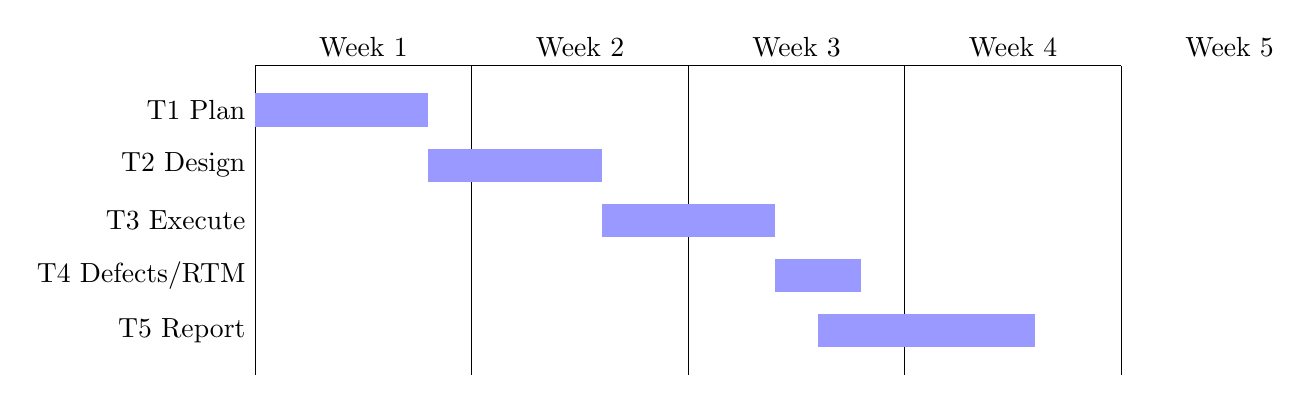
\begin{tikzpicture}[x=0.55cm,y=0.7cm]
  \foreach \w in {0,1,2,3,4} { \draw (\w*5,0.3) -- (\w*5,-5.3); \node[above] at (\w*5+2.5,0.3) {Week \the\numexpr\w+1\relax}; }
  \draw (0,0.3) -- (20,0.3);
  \node[left] at (0,-0.5) {T1 Plan};        \fill[blue!40] (0,-0.8) rectangle (4,-0.2);
  \node[left] at (0,-1.5) {T2 Design};      \fill[blue!40] (4,-1.8) rectangle (8,-1.2);
  \node[left] at (0,-2.5) {T3 Execute};     \fill[blue!40] (8,-2.8) rectangle (12,-2.2);
  \node[left] at (0,-3.5) {T4 Defects/RTM}; \fill[blue!40] (12,-3.8) rectangle (14,-3.2);
  \node[left] at (0,-4.5) {T5 Report};      \fill[blue!40] (13,-4.8) rectangle (18,-4.2);
\end{tikzpicture}
\caption{Project timeline (Gantt chart)}
\label{fig:gantt}
\end{figure}
Please refer to Annexure C for the planner.

\section{Team Organization}
\subsection{Team structure}
Four students: one test lead (plan, RTM, review), one responsible for login and products cases, one for cart and checkout cases, one for defect reports and evidence. All members executed cases and cross-checked each other's results.

\subsection{Management reporting and communication}
Weekly review with the guide in the LP-IV slot; a shared GitHub repository holds all artifacts; a group chat for daily coordination.

% =====================================================================
\chapter{Software requirement specification}

\section{Introduction}
\subsection{Purpose and Scope of Document}
This SRS summarises the functional requirements of the application under test (Swag Labs) as understood by the test team, so that test cases can be derived from them and traced back.

\subsection{Overview of responsibilities of Developer}
In this project the team acts as the QA team: derive requirements from the application, design and execute tests, and report defects. Fixing defects is the responsibility of the application's developers (Sauce Labs).

\section{Usage Scenario}
\subsection{User profiles}
\begin{itemize}
  \item \textbf{Customer:} logs in, browses products, manages the cart and places an order.
  \item \textbf{Tester:} executes test cases as each of the six test users and records results.
  \item \textbf{Test lead:} reviews cases, maintains RTM and defect status.
\end{itemize}

\subsection{Use-cases}
\begin{table}[H]
\begin{center}
\def\arraystretch{1.5}
\begin{tabularx}{\textwidth}{| c | l | X | c | X |}
\hline
Sr No.	& Use Case	& Description	& Actors	& Assumptions \\
\hline
1& Login & Authenticate with username and password & Customer & Test user accounts exist \\
\hline
2& Browse / sort products & View six products and sort by name or price & Customer & Logged in \\
\hline
3& Manage cart & Add, remove, view items; badge shows count & Customer & Logged in \\
\hline
4& Checkout & Enter name and postal code, review totals, finish order & Customer & Cart not empty \\
\hline
5& Logout / navigate & Use side menu, logout, reset app state & Customer & Logged in \\
\hline
6& Execute test case & Perform steps, compare actual vs expected, record status & Tester & Test case sheet ready \\
\hline
7& Report defect & Log a failure with steps, severity, priority and evidence & Tester & A test case failed \\
\hline
\end{tabularx}
\end{center}
\caption{Use Cases}
\label{tab:usecase}
\end{table}

\subsection{Use Case View}
\begin{figure}[H]
\centering
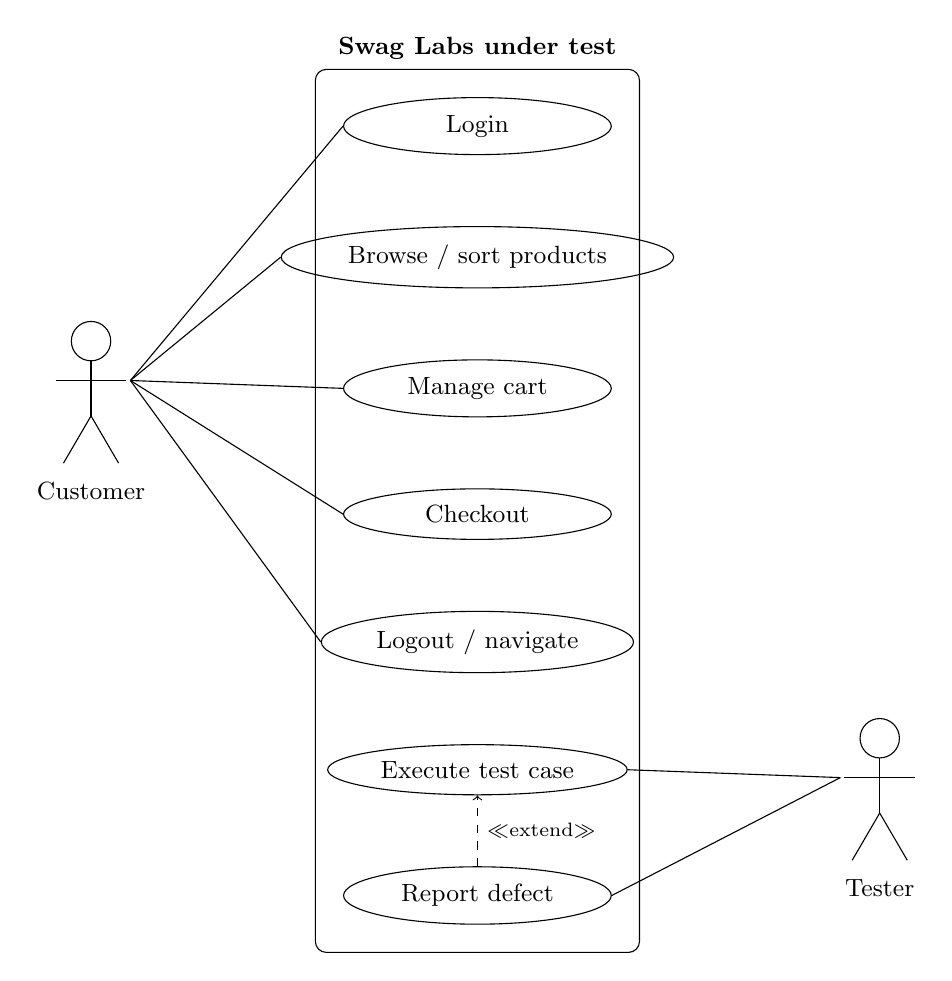
\begin{tikzpicture}[node distance=0.9cm, every node/.style={font=\small}]
  \node[draw, ellipse, minimum width=3.4cm] (u1) {Login};
  \node[draw, ellipse, minimum width=3.4cm, below=of u1] (u2) {Browse / sort products};
  \node[draw, ellipse, minimum width=3.4cm, below=of u2] (u3) {Manage cart};
  \node[draw, ellipse, minimum width=3.4cm, below=of u3] (u4) {Checkout};
  \node[draw, ellipse, minimum width=3.4cm, below=of u4] (u5) {Logout / navigate};
  \node[draw, ellipse, minimum width=3.4cm, below=of u5] (u6) {Execute test case};
  \node[draw, ellipse, minimum width=3.4cm, below=of u6] (u7) {Report defect};
  \node[draw, rounded corners, fit=(u1)(u7), inner sep=10pt, label=above:{\textbf{Swag Labs under test}}] (sys) {};
  % customer actor (left)
  \coordinate (ch) at ($(u3.west)+(-3.2cm,0.6cm)$);
  \draw (ch) circle (0.25);
  \draw ($(ch)+(0,-0.25)$) -- ++(0,-0.7);
  \draw ($(ch)+(-0.45,-0.5)$) -- ++(0.9,0);
  \draw ($(ch)+(0,-0.95)$) -- ++(-0.35,-0.6);
  \draw ($(ch)+(0,-0.95)$) -- ++(0.35,-0.6);
  \node at ($(ch)+(0,-1.9)$) {Customer};
  \coordinate (cact) at ($(ch)+(0.5,-0.5)$);
  \foreach \u in {u1,u2,u3,u4,u5} \draw (cact) -- (\u.west);
  % tester actor (right)
  \coordinate (th) at ($(u6.east)+(3.2cm,0.4cm)$);
  \draw (th) circle (0.25);
  \draw ($(th)+(0,-0.25)$) -- ++(0,-0.7);
  \draw ($(th)+(-0.45,-0.5)$) -- ++(0.9,0);
  \draw ($(th)+(0,-0.95)$) -- ++(-0.35,-0.6);
  \draw ($(th)+(0,-0.95)$) -- ++(0.35,-0.6);
  \node at ($(th)+(0,-1.9)$) {Tester};
  \coordinate (tact) at ($(th)+(-0.5,-0.5)$);
  \foreach \u in {u6,u7} \draw (tact) -- (\u.east);
  \draw[dashed,->] (u7) -- (u6) node[midway,right] {\scriptsize $\ll$extend$\gg$};
\end{tikzpicture}
\caption{Use case diagram}
\label{fig:usecase}
\end{figure}

\section{Data Model and Description}
\subsection{Data Description}
The testing artifacts are tabular: Test Case (ID, module, title, pre-condition, steps, test data, expected, actual, status, priority, defect ID, evidence); Defect (ID, summary, module, severity, priority, status, steps, expected, actual, test case, evidence); Requirement (ID, description, test cases).

\subsection{Data objects and Relationships}
\begin{figure}[H]
\centering
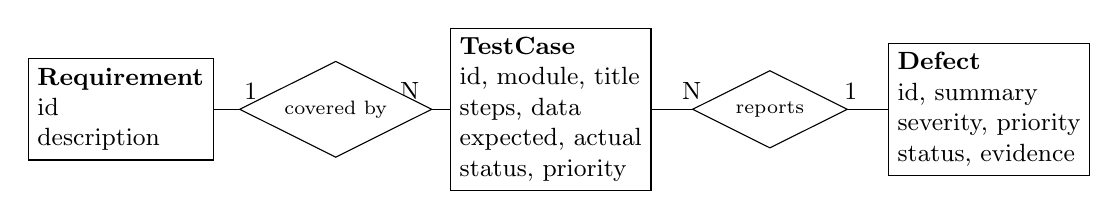
\begin{tikzpicture}[every node/.style={font=\small}]
  \node[draw, rectangle, align=left] (req) {\textbf{Requirement}\\ id\\ description};
  \node[draw, rectangle, align=left, right=3cm of req] (tc) {\textbf{TestCase}\\ id, module, title\\ steps, data\\ expected, actual\\ status, priority};
  \node[draw, rectangle, align=left, right=3cm of tc] (def) {\textbf{Defect}\\ id, summary\\ severity, priority\\ status, evidence};
  \draw (req) -- node[above] {1 \hspace{1.6cm} N} (tc);
  \node[draw, diamond, aspect=2, fill=white, font=\scriptsize] at ($(req)!0.5!(tc)$) {covered by};
  \draw (tc) -- node[above] {N \hspace{1.6cm} 1} (def);
  \node[draw, diamond, aspect=2, fill=white, font=\scriptsize] at ($(tc)!0.5!(def)$) {reports};
\end{tikzpicture}
\caption{Entity relationship of test artifacts}
\label{fig:erd}
\end{figure}

\section{Functional Model and Description}
\subsection{Data Flow Diagram}
\subsubsection{Level 0 Data Flow Diagram}
\begin{figure}[H]
\centering
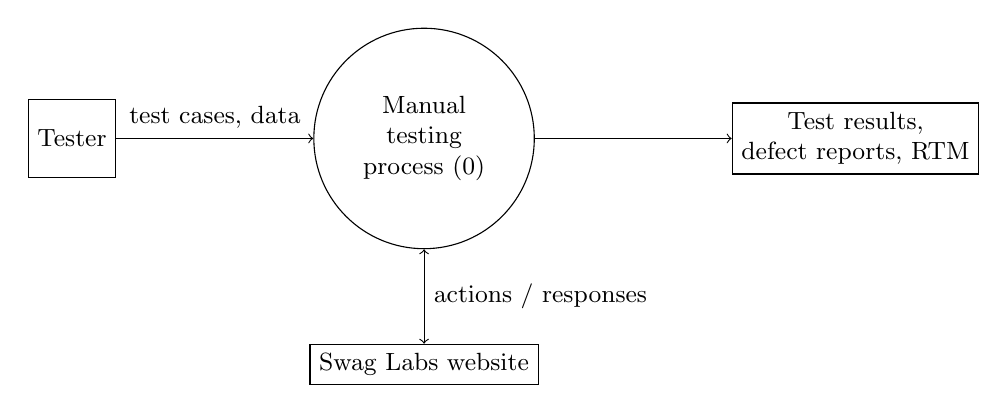
\begin{tikzpicture}[node distance=2.5cm, every node/.style={font=\small}]
  \node[draw, rectangle, minimum height=1cm] (t) {Tester};
  \node[draw, circle, minimum size=2.8cm, align=center, right=of t] (p) {Manual\\testing\\process (0)};
  \node[draw, rectangle, align=center, right=of p] (out) {Test results,\\defect reports, RTM};
  \node[draw, rectangle, below=1.2cm of p] (app) {Swag Labs website};
  \draw[->] (t) -- node[above] {test cases, data} (p);
  \draw[<->] (app) -- node[right] {actions / responses} (p);
  \draw[->] (p) -- (out);
\end{tikzpicture}
\caption{Level 0 DFD}
\label{fig:dfd0}
\end{figure}

\subsubsection{Level 1 Data Flow Diagram}
\begin{figure}[H]
\centering
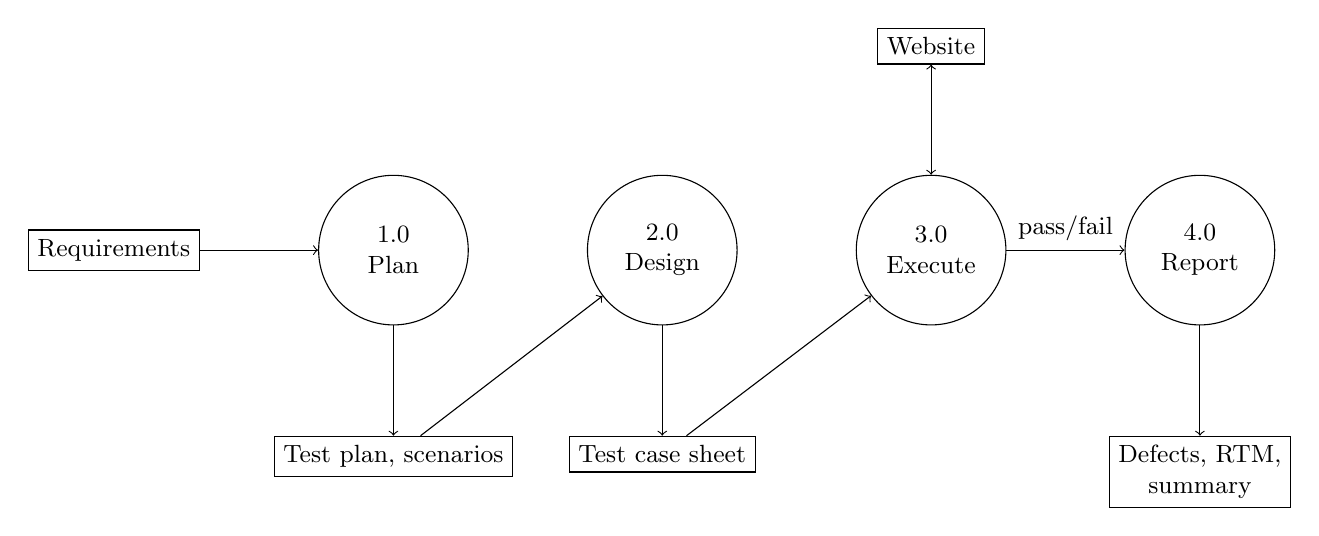
\begin{tikzpicture}[node distance=1.4cm and 1.5cm, every node/.style={font=\small}]
  \node[draw, rectangle] (req) {Requirements};
  \node[draw, circle, minimum size=1.9cm, align=center, right=of req] (p1) {1.0\\Plan};
  \node[draw, circle, minimum size=1.9cm, align=center, right=of p1] (p2) {2.0\\Design};
  \node[draw, circle, minimum size=1.9cm, align=center, right=of p2] (p3) {3.0\\Execute};
  \node[draw, circle, minimum size=1.9cm, align=center, right=of p3] (p4) {4.0\\Report};
  \node[draw, rectangle, below=of p1] (plan) {Test plan, scenarios};
  \node[draw, rectangle, below=of p2] (sheet) {Test case sheet};
  \node[draw, rectangle, above=of p3] (app) {Website};
  \node[draw, rectangle, below=of p4, align=center] (out) {Defects, RTM,\\summary};
  \draw[->] (req) -- (p1); \draw[->] (p1) -- (plan); \draw[->] (plan) -- (p2); \draw[->] (p2) -- (sheet);
  \draw[->] (sheet) -- (p3); \draw[<->] (p3) -- (app); \draw[->] (p3) -- node[above] {pass/fail} (p4); \draw[->] (p4) -- (out);
\end{tikzpicture}
\caption{Level 1 DFD}
\label{fig:dfd1}
\end{figure}

\subsection{Activity Diagram:}
\begin{figure}[H]
\centering
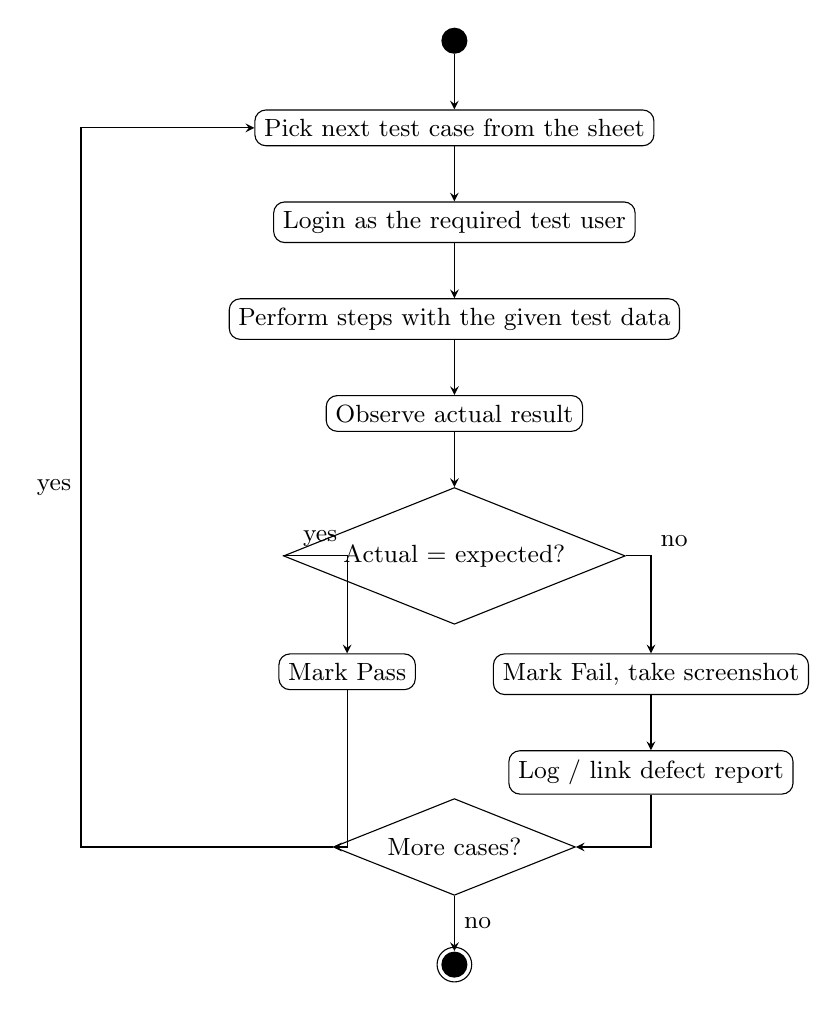
\begin{tikzpicture}[node distance=0.7cm, every node/.style={font=\small}, >=stealth]
  \node[circle, fill=black, minimum size=0.3cm] (s) {};
  \node[draw, rounded corners, below=of s] (a1) {Pick next test case from the sheet};
  \node[draw, rounded corners, below=of a1] (a2) {Login as the required test user};
  \node[draw, rounded corners, below=of a2] (a3) {Perform steps with the given test data};
  \node[draw, rounded corners, below=of a3] (a4) {Observe actual result};
  \node[draw, diamond, aspect=2.5, below=of a4] (d1) {Actual = expected?};
  \node[draw, rounded corners, below left=0.8cm and -0.6cm of d1] (p) {Mark Pass};
  \node[draw, rounded corners, below right=0.8cm and -0.6cm of d1] (f) {Mark Fail, take screenshot};
  \node[draw, rounded corners, below=of f] (df) {Log / link defect report};
  \node[draw, diamond, aspect=2.5, below=2.2cm of d1] (d2) {More cases?};
  \node[circle, fill=black, minimum size=0.3cm, below=of d2] (e) {};
  \draw (e) circle (0.22cm);
  \draw[->] (s) -- (a1); \draw[->] (a1) -- (a2); \draw[->] (a2) -- (a3); \draw[->] (a3) -- (a4); \draw[->] (a4) -- (d1);
  \draw[->] (d1) -| node[above left] {yes} (p); \draw[->] (d1) -| node[above right] {no} (f); \draw[->] (f) -- (df);
  \draw[->] (p) |- (d2); \draw[->] (df) |- (d2);
  \draw[->] (d2) -- node[right] {no} (e);
  \draw[->] (d2.west) -- ++(-3.2,0) |- node[pos=0.25, left] {yes} (a1.west);
\end{tikzpicture}
\caption{Activity diagram of test execution}
\label{fig:activity}
\end{figure}

\subsection{Non Functional Requirements:}
\begin{itemize}
  \item \textbf{Interface Requirements:} the website is used through a standard desktop browser; artifacts are Excel and Markdown files readable without special tools.
  \item \textbf{Performance Requirements:} pages should load within 3 seconds (used as the pass criterion for the performance test case).
  \item \textbf{Availability:} testing depends on the public site being reachable.
  \item \textbf{Modifiability:} the workbook is generated from one data file so test cases can be edited and regenerated.
  \item \textbf{Security:} protected pages must not open without login (verified by TC\_MENU\_03).
  \item \textbf{Testability / Usability:} every case lists exact steps and data so that any tester reproduces the same result.
\end{itemize}

\subsection{State Diagram:}
Fig.\ref{fig:state-dig} shows the defect life cycle used for the Status column of the defect sheet.
\begin{figure}[H]
\centering
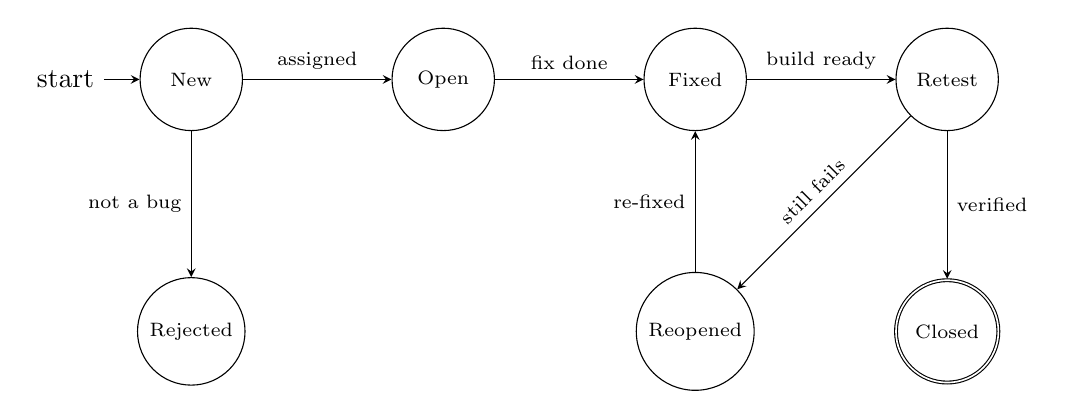
\begin{tikzpicture}[->, >=stealth, node distance=3.2cm, every state/.style={font=\scriptsize, minimum size=1.3cm}]
  \node[state, initial] (new) {New};
  \node[state, right of=new] (open) {Open};
  \node[state, right of=open] (fixed) {Fixed};
  \node[state, right of=fixed] (retest) {Retest};
  \node[state, accepting, below of=retest] (closed) {Closed};
  \node[state, below of=new] (rej) {Rejected};
  \node[state, below of=fixed] (reopen) {Reopened};
  \path (new) edge node[above, font=\scriptsize] {assigned} (open)
        (open) edge node[above, font=\scriptsize] {fix done} (fixed)
        (fixed) edge node[above, font=\scriptsize] {build ready} (retest)
        (retest) edge node[right, font=\scriptsize] {verified} (closed)
        (retest) edge node[above, sloped, font=\scriptsize] {still fails} (reopen)
        (reopen) edge node[left, font=\scriptsize] {re-fixed} (fixed)
        (new) edge node[left, font=\scriptsize] {not a bug} (rej);
\end{tikzpicture}
\caption{State transition diagram (defect life cycle)}
\label{fig:state-dig}
\end{figure}

\subsection{Design Constraints}
Test cases must be executable by hand without tools; every Fail must carry evidence; the workbook format must be plain Excel.

\subsection{Software Interface Description}
\begin{itemize}
  \item \textbf{Application interface:} HTTPS web pages of Swag Labs in Microsoft Edge.
  \item \textbf{Artifact interface:} Excel workbook (openpyxl), Markdown files, PNG screenshots.
\end{itemize}

% =====================================================================
\chapter{Detailed Design Document using Appendix A and B}
\section{Introduction}
This chapter describes the structure of the testing process and of the artifacts produced.

\section{Architectural Design}
\begin{figure}[H]
\centering
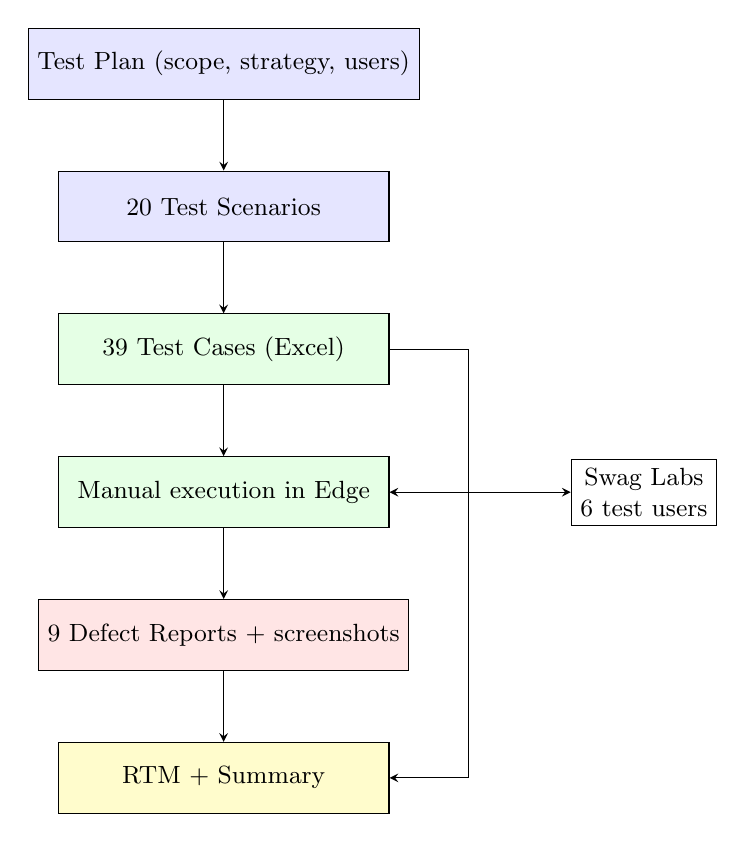
\begin{tikzpicture}[node distance=0.9cm, every node/.style={font=\small}, >=stealth]
  \node[draw, fill=blue!10, minimum width=4.2cm, minimum height=0.9cm] (plan) {Test Plan (scope, strategy, users)};
  \node[draw, fill=blue!10, minimum width=4.2cm, minimum height=0.9cm, below=of plan] (scen) {20 Test Scenarios};
  \node[draw, fill=green!10, minimum width=4.2cm, minimum height=0.9cm, below=of scen] (tc) {39 Test Cases (Excel)};
  \node[draw, fill=green!10, minimum width=4.2cm, minimum height=0.9cm, below=of tc] (exec) {Manual execution in Edge};
  \node[draw, fill=red!10, minimum width=4.2cm, minimum height=0.9cm, below=of exec] (def) {9 Defect Reports + screenshots};
  \node[draw, fill=yellow!20, minimum width=4.2cm, minimum height=0.9cm, below=of def] (rtm) {RTM + Summary};
  \node[draw, right=2.3cm of exec, align=center] (site) {Swag Labs\\6 test users};
  \draw[->] (plan) -- (scen); \draw[->] (scen) -- (tc); \draw[->] (tc) -- (exec); \draw[->] (exec) -- (def); \draw[->] (def) -- (rtm);
  \draw[<->] (exec) -- (site);
  \draw[->] (tc.east) -- ++(1.0,0) |- (rtm.east);
\end{tikzpicture}
\caption{Architecture of the testing process}
\label{fig:arch-dig}
\end{figure}

\section{Data design (using Appendices A and B)}
\subsection{Internal software data structure}
Each test case is a 12-field record; each defect an 11-field record; each requirement a 3-field record (see Chapter 6). The records are kept in one Python list each inside \texttt{tools/build\_documents.py}.
\subsection{Global data structure}
The site URL, the common password and the severity/priority scales are global constants used by all records.
\subsection{Temporary data structure}
Counters for pass/fail per module used to build the Summary sheet.
\subsection{Database description}
No database; the Excel workbook \texttt{SwagLabs\_Test\_Cases.xlsx} with sheets Test Cases, Defect Reports, RTM and Summary is the persistent store.

\section{Component Design}
\subsection{Class Diagram}
\begin{figure}[H]
\centering
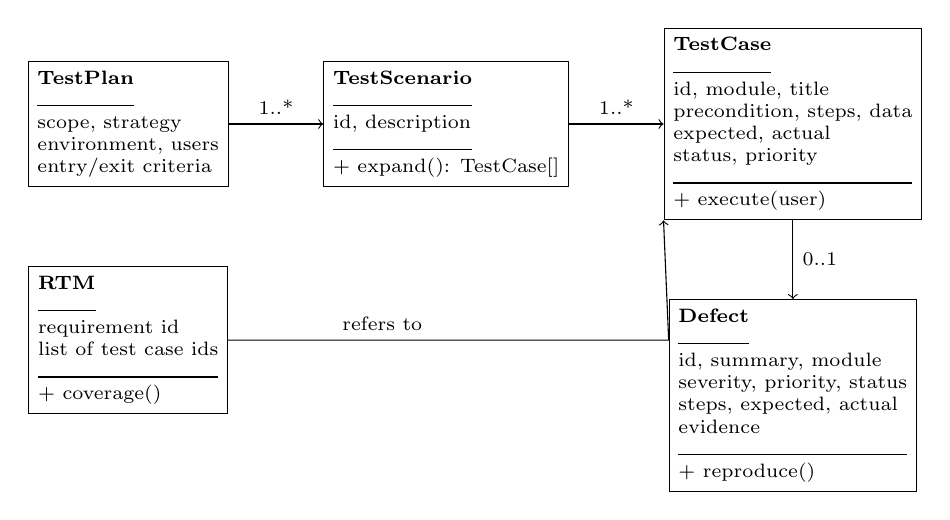
\begin{tikzpicture}[node distance=1.0cm and 1.2cm, every node/.style={font=\scriptsize}]
  \node[draw, rectangle, align=left] (tp) {\textbf{TestPlan}\\ \hrulefill\\ scope, strategy\\ environment, users\\ entry/exit criteria};
  \node[draw, rectangle, align=left, right=of tp] (ts) {\textbf{TestScenario}\\ \hrulefill\\ id, description\\ \hrulefill\\ + expand(): TestCase[]};
  \node[draw, rectangle, align=left, right=of ts] (tc) {\textbf{TestCase}\\ \hrulefill\\ id, module, title\\ precondition, steps, data\\ expected, actual\\ status, priority\\ \hrulefill\\ + execute(user)};
  \node[draw, rectangle, align=left, below=of tc] (d) {\textbf{Defect}\\ \hrulefill\\ id, summary, module\\ severity, priority, status\\ steps, expected, actual\\ evidence\\ \hrulefill\\ + reproduce()};
  \node[draw, rectangle, align=left, below=of tp] (r) {\textbf{RTM}\\ \hrulefill\\ requirement id\\ list of test case ids\\ \hrulefill\\ + coverage()};
  \draw[->] (tp) -- node[above] {1..*} (ts);
  \draw[->] (ts) -- node[above] {1..*} (tc);
  \draw[->] (tc) -- node[right] {0..1} (d);
  \draw[->] (r.east) -- node[above, pos=0.35] {refers to} (d.west |- r.east) -- (tc.south west);
\end{tikzpicture}
\caption{Class diagram of test artifacts}
\label{fig:class-dig}
\end{figure}

% =====================================================================
\chapter{Project Implementation}
\section{Introduction}
The project was implemented as a set of documents and an Excel workbook, supported by two small Python scripts: one that builds the workbook and Markdown files from a single data set, and one that re-captures the evidence screenshots. Repository: \url{https://github.com/VishwajeetTulse/ecommerce-manual-testing}.

\section{Tools and Technologies Used}
\begin{itemize}
  \item Microsoft Edge 142 on Windows 11 for execution
  \item Microsoft Excel (workbook produced with Python \texttt{openpyxl})
  \item Python 3.14 with \texttt{openpyxl} and \texttt{selenium} (evidence re-capture only)
  \item Git and GitHub; MiKTeX for this report
\end{itemize}

\section{Methodologies/Algorithm Details}
\subsection{Algorithm 1/Pseudo Code}
\begin{algorithm}[H]
\caption{Test case design from a requirement}
\KwIn{requirement $r$, its input fields $F$}
\KwOut{set of test cases $TC_r$}
add one positive case covering the normal flow of $r$\;
\ForEach{field $f \in F$}{
  partition the domain of $f$ into valid and invalid classes\;
  add one case per invalid class (empty, wrong type, wrong format)\;
  add boundary cases where $f$ has limits\;
}
\ForEach{special test user $u$ relevant to $r$}{add an error-guessing case executed as $u$\;}
record $(r, tc)$ in the RTM for every $tc \in TC_r$\;
\Return $TC_r$\;
\end{algorithm}

\subsection{Algorithm 2/Pseudo Code}
\begin{algorithm}[H]
\caption{Manual execution and defect logging}
\KwIn{test case sheet $TC$}
\KwOut{status for each case, defect list $D$}
\ForEach{$tc \in TC$ grouped by test user}{
  log in as the required user; establish the pre-condition\;
  perform the steps with the given test data; observe the actual result\;
  \eIf{actual = expected}{status $\leftarrow$ Pass}{
    status $\leftarrow$ Fail; capture screenshot\;
    \eIf{an existing defect $d \in D$ matches}{link $tc$ to $d$}{create new defect with severity, priority, steps, expected, actual, evidence; add to $D$}
  }
}
compute pass percentage and module-wise summary\;
\end{algorithm}

Example of a designed test case (checkout postal code, invalid equivalence class):
\begin{lstlisting}
TC_CHK_06  Module: Checkout   Priority: Medium
Pre-condition : cart has items; on "Checkout: Your Information"
Steps         : 1. Enter First Name "Vishwajeet"  2. Enter Last Name "Tulse"
                3. Enter Postal Code "abc"        4. Click Continue
Expected      : validation error for Postal Code
Actual        : form accepted, Overview page displayed
Status        : Fail   -> DEF-05
\end{lstlisting}

\section{Verification and Validation for Acceptance}
Acceptance criteria for the test package: every requirement has at least one test case (RTM complete); every test case has an actual result and status; every Fail is linked to a defect with a screenshot; the summary totals equal the sheet counts. All criteria were checked by the test lead; the summary sheet is generated automatically from the same data as the test-case sheet, so the counts cannot disagree.

% =====================================================================
\chapter{Software Testing}
\section{Type of Testing Used}
\begin{itemize}
  \item \textbf{Functional testing} of each feature (login, products, cart, checkout, navigation).
  \item \textbf{Negative testing} with empty, invalid and locked-out inputs.
  \item \textbf{UI testing} of elements, labels, alignment and button states.
  \item \textbf{System testing} of the end-to-end purchase flow.
  \item \textbf{Regression}: the full sheet was executed twice; the second run found that a new menu link had been added to the site and TC\_MENU\_01 was updated.
\end{itemize}

\section{Test Cases and Test Results}
\begin{table}[H]
\begin{center}
\def\arraystretch{1.3}
\begin{tabular}{| l | c | c | c |}
\hline
Module & Test cases & Pass & Fail \\ \hline
Login & 8 & 7 & 1 \\ \hline
Products & 8 & 3 & 5 \\ \hline
Cart & 6 & 4 & 2 \\ \hline
Checkout & 11 & 8 & 3 \\ \hline
Menu & 3 & 3 & 0 \\ \hline
UI & 3 & 3 & 0 \\ \hline
\textbf{Total} & \textbf{39} & \textbf{28} & \textbf{11} \\ \hline
\end{tabular}
\caption{Module-wise test results (pass percentage 71.8\%)}
\label{tab:summary}
\end{center}
\end{table}

\begin{table}[H]
\begin{center}
\def\arraystretch{1.3}
\begin{tabularx}{\textwidth}{| l | X | l | c |}
\hline
TC & Title & User & Status \\ \hline
TC\_LOGIN\_03 & Login with valid credentials & standard\_user & Pass \\ \hline
TC\_LOGIN\_04 & Login with empty username and password & -- & Pass \\ \hline
TC\_LOGIN\_06 & Login with locked-out user & locked\_out\_user & Pass \\ \hline
TC\_LOGIN\_08 & Login response time & performance\_glitch\_user & Fail \\ \hline
TC\_PROD\_02 & Sort products by price low to high & standard\_user & Pass \\ \hline
TC\_PROD\_04 & Product images match the product & problem\_user & Fail \\ \hline
TC\_PROD\_05 & Sort by price works & problem\_user & Fail \\ \hline
TC\_PROD\_06 & Sort dropdown works & error\_user & Fail \\ \hline
TC\_PROD\_07 & Prices match the catalogue & visual\_user & Fail \\ \hline
TC\_CART\_01 & Add two products and verify badge & standard\_user & Pass \\ \hline
TC\_CART\_04 & Add to cart works for all products & problem\_user & Fail \\ \hline
TC\_CART\_05 & Cart is cleared on logout & standard\_user & Fail \\ \hline
TC\_CHK\_01 & Checkout with empty information form & standard\_user & Pass \\ \hline
TC\_CHK\_05 & First name rejects numeric input & standard\_user & Fail \\ \hline
TC\_CHK\_06 & Postal code rejects alphabetic input & standard\_user & Fail \\ \hline
TC\_CHK\_07 & Overview totals, tax 8\% and total & standard\_user & Pass \\ \hline
TC\_CHK\_09 & Finish order shows confirmation & standard\_user & Pass \\ \hline
TC\_CHK\_10 & Last Name field accepts input & problem\_user & Fail \\ \hline
TC\_MENU\_03 & Protected page cannot be opened without login & -- & Pass \\ \hline
\end{tabularx}
\end{center}
\caption{Selected test cases (full list of 39 in the Excel workbook)}
\label{tab:tests}
\end{table}

\begin{table}[H]
\begin{center}
\def\arraystretch{1.3}
\begin{tabularx}{\textwidth}{| l | X | l | l |}
\hline
ID & Summary & Severity & Priority \\ \hline
DEF-01 & Wrong product images for problem\_user & High & Medium \\ \hline
DEF-02 & Price sorting does not reorder products for problem\_user & Medium & Medium \\ \hline
DEF-03 & Add to cart has no effect for some products (problem\_user) & High & High \\ \hline
DEF-04 & Last Name field cannot be filled during checkout (problem\_user) & Critical & High \\ \hline
DEF-05 & Checkout form accepts invalid data (all users) & Medium & Medium \\ \hline
DEF-06 & Cart contents persist after logout and re-login & Medium & Low \\ \hline
DEF-07 & Sorting shows a JavaScript alert for error\_user & Medium & Medium \\ \hline
DEF-08 & Login takes about 7 seconds for performance\_glitch\_user & Medium & Low \\ \hline
DEF-09 & Wrong prices and misaligned layout for visual\_user & High & Medium \\ \hline
\end{tabularx}
\end{center}
\caption{Defects logged}
\label{tab:defects}
\end{table}

% =====================================================================
\chapter{Results}
\section{Screen shots}
\begin{figure}[H]
\centering
\fbox{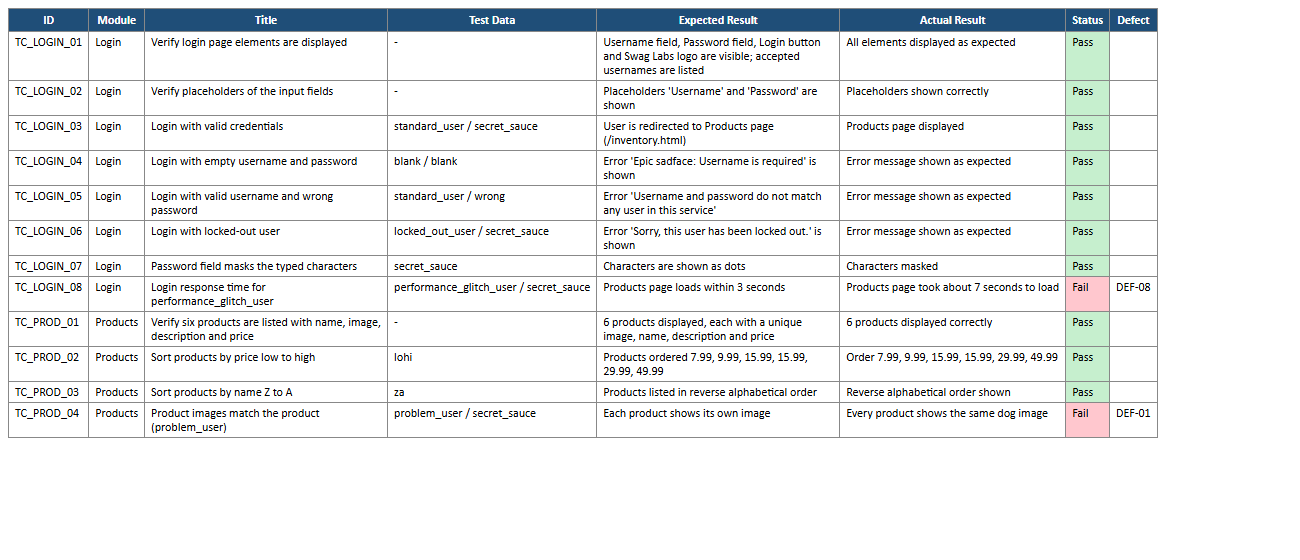
\includegraphics[width=0.95\textwidth]{figures/excel_preview.png}}
\caption{Test case sheet (first rows of the Excel workbook)}
\end{figure}
\begin{figure}[H]
\centering
\fbox{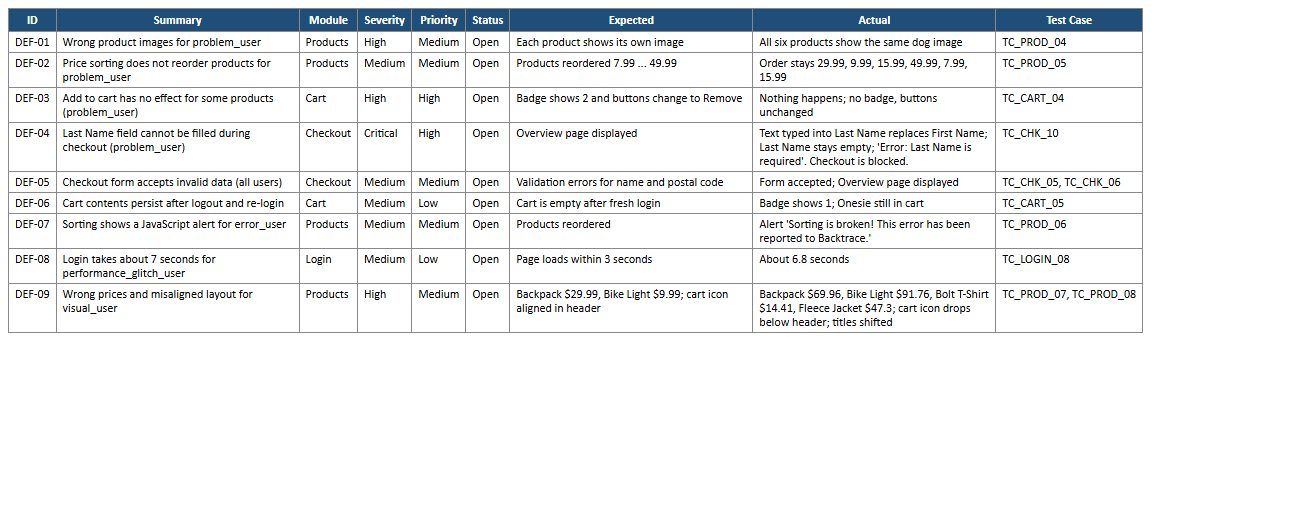
\includegraphics[width=0.95\textwidth]{figures/defect_preview.png}}
\caption{Defect report sheet}
\end{figure}
\begin{figure}[H]
\centering
\begin{subfigure}{0.48\textwidth}
\fbox{
\includegraphics[width=\textwidth]{../screenshots/01_login_page.png}}
\caption{Login page (TC\_LOGIN\_01)}
\end{subfigure}
\hfill
\begin{subfigure}{0.48\textwidth}
\fbox{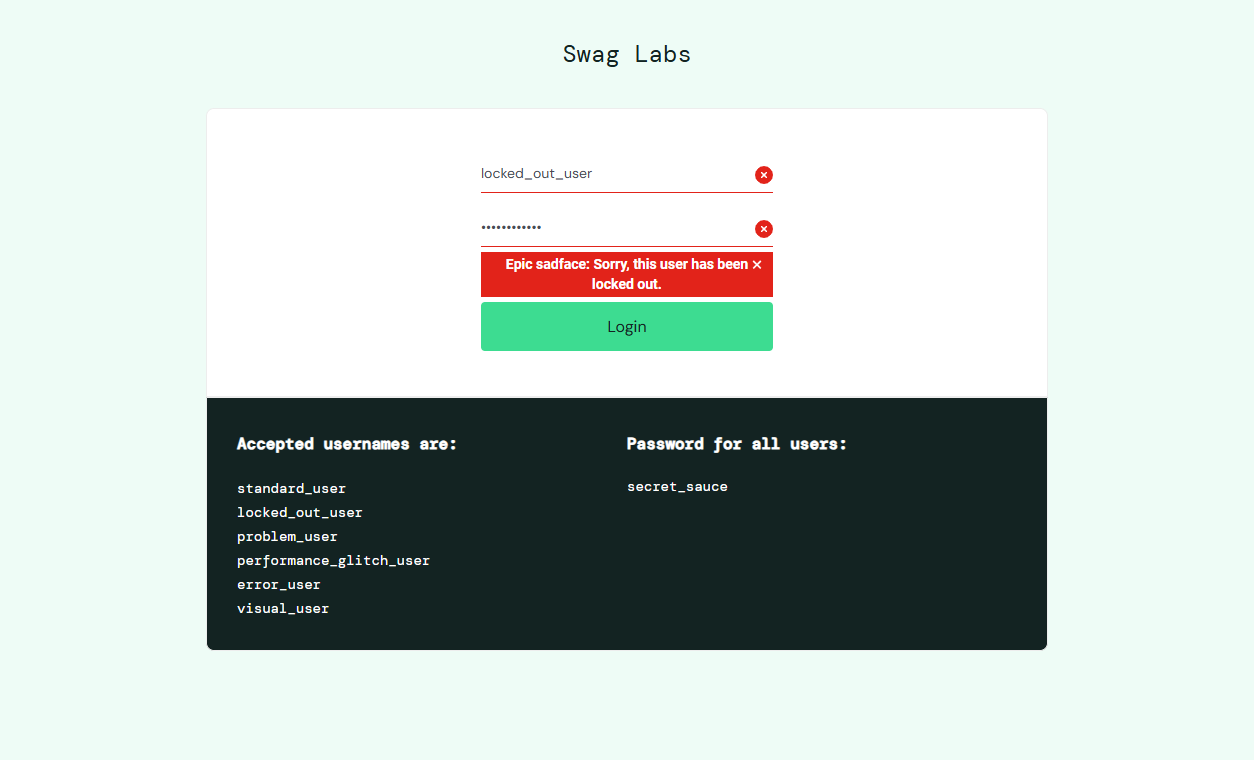
\includegraphics[width=\textwidth]{../screenshots/03_locked_out_user_error.png}}
\caption{Locked-out user error (TC\_LOGIN\_06)}
\end{subfigure}
\caption{Login test evidence}
\end{figure}
\begin{figure}[H]
\centering
\begin{subfigure}{0.48\textwidth}
\fbox{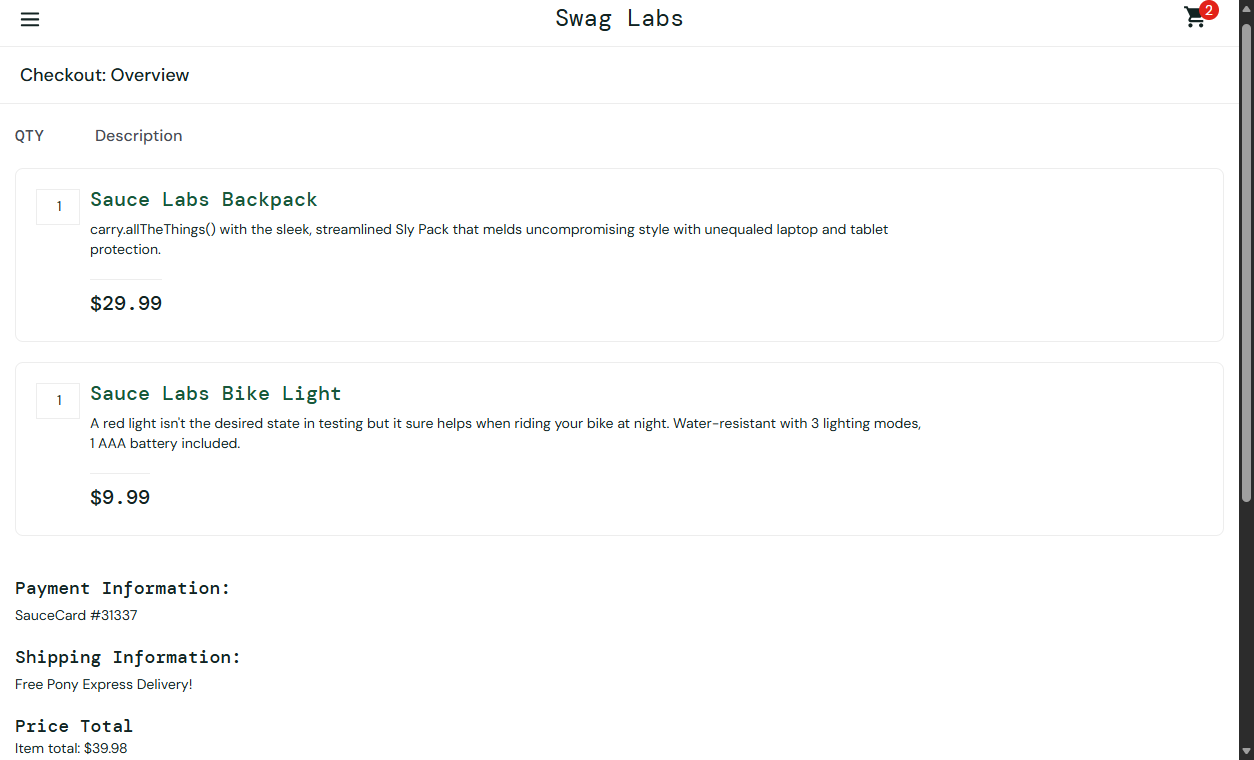
\includegraphics[width=\textwidth]{../screenshots/11_checkout_overview.png}}
\caption{Checkout overview, totals correct (TC\_CHK\_07)}
\end{subfigure}
\hfill
\begin{subfigure}{0.48\textwidth}
\fbox{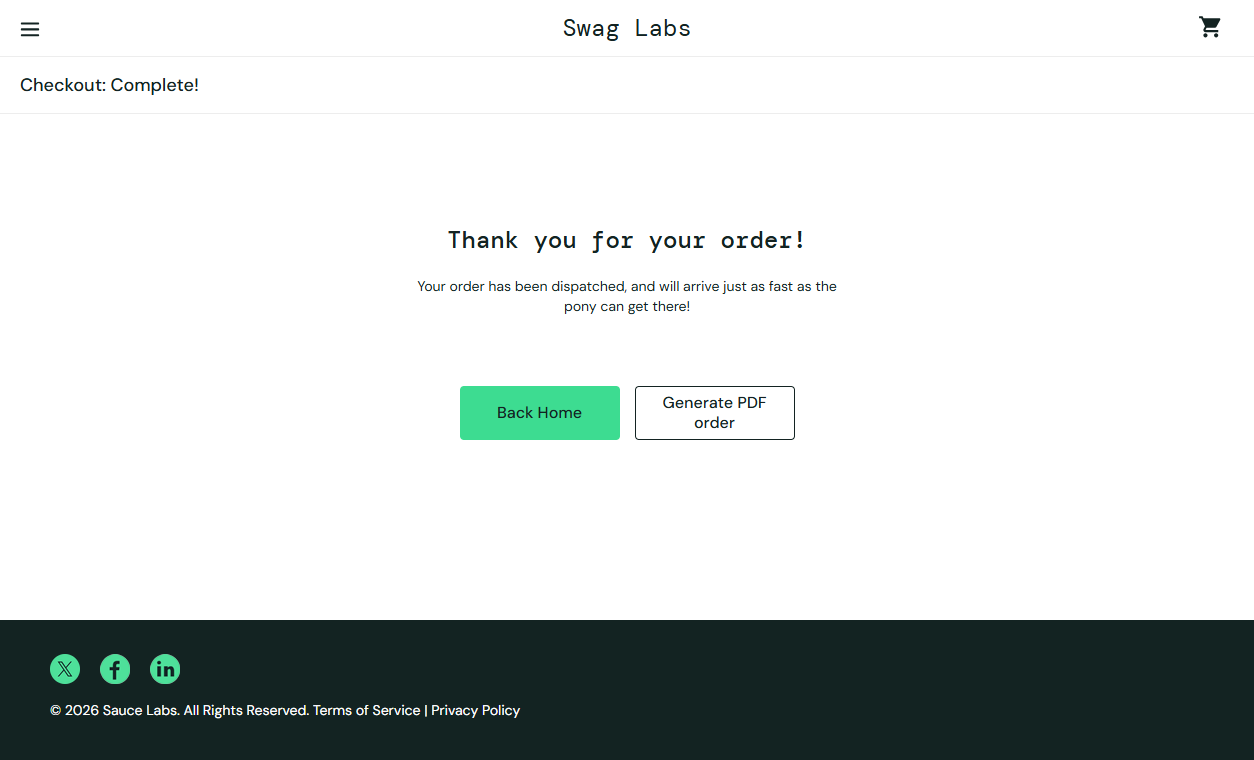
\includegraphics[width=\textwidth]{../screenshots/12_order_complete.png}}
\caption{Order complete (TC\_CHK\_09)}
\end{subfigure}
\caption{Checkout happy-path evidence}
\end{figure}
\begin{figure}[H]
\centering
\begin{subfigure}{0.48\textwidth}
\fbox{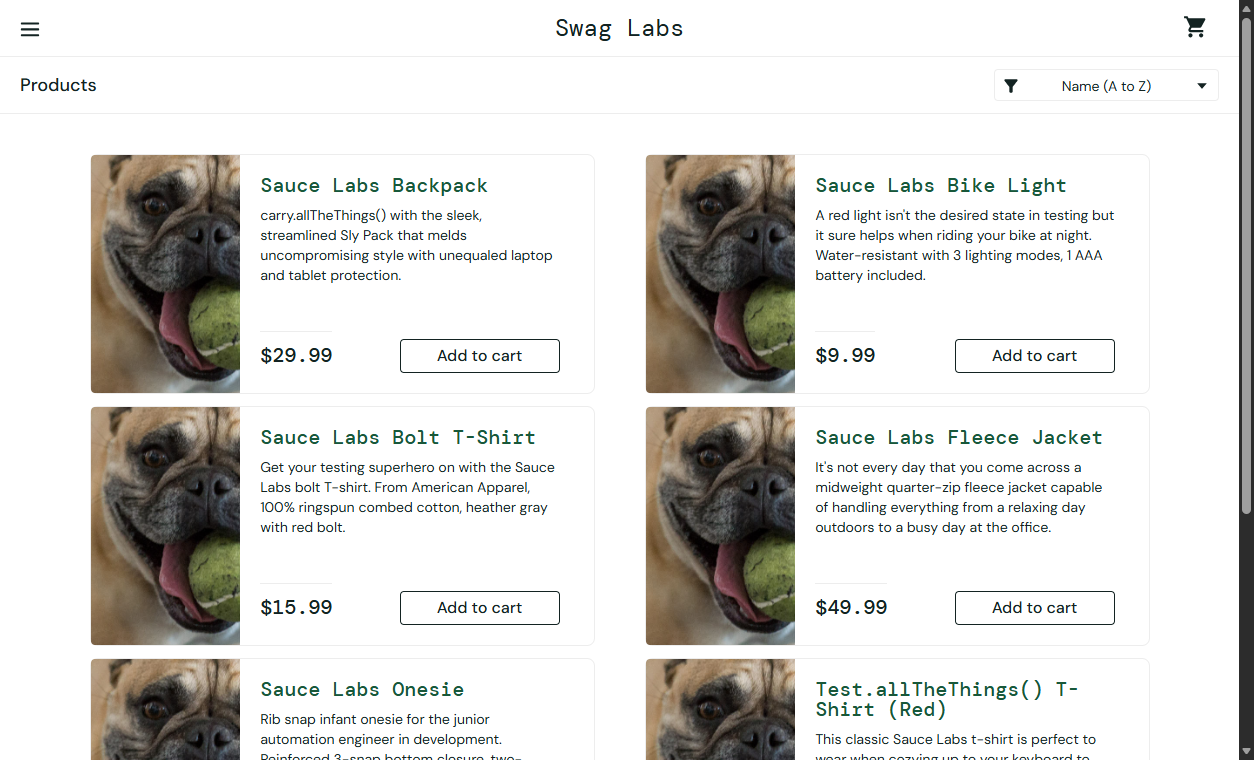
\includegraphics[width=\textwidth]{../screenshots/15_problem_user_same_images.png}}
\caption{DEF-01 wrong product images}
\end{subfigure}
\hfill
\begin{subfigure}{0.48\textwidth}
\fbox{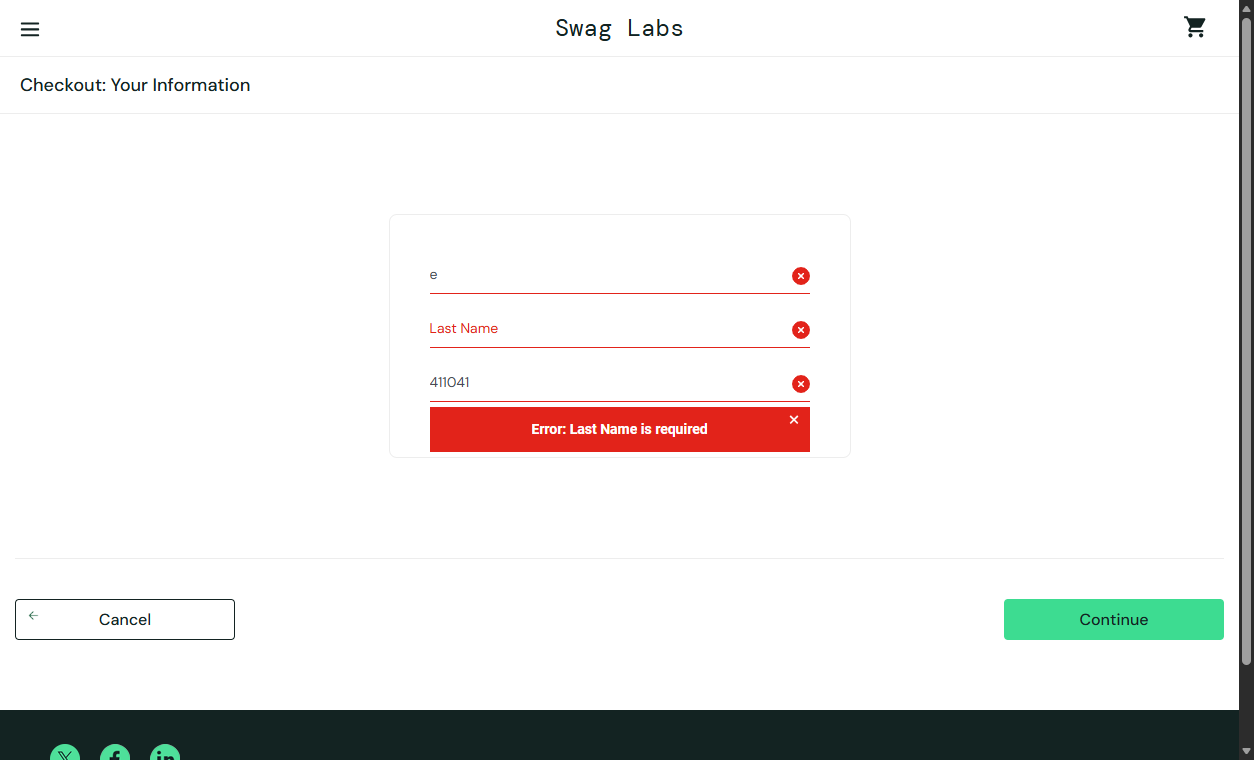
\includegraphics[width=\textwidth]{../screenshots/18_problem_user_lastname_bug.png}}
\caption{DEF-04 Last Name cannot be filled}
\end{subfigure}
\\[4pt]
\begin{subfigure}{0.48\textwidth}
\fbox{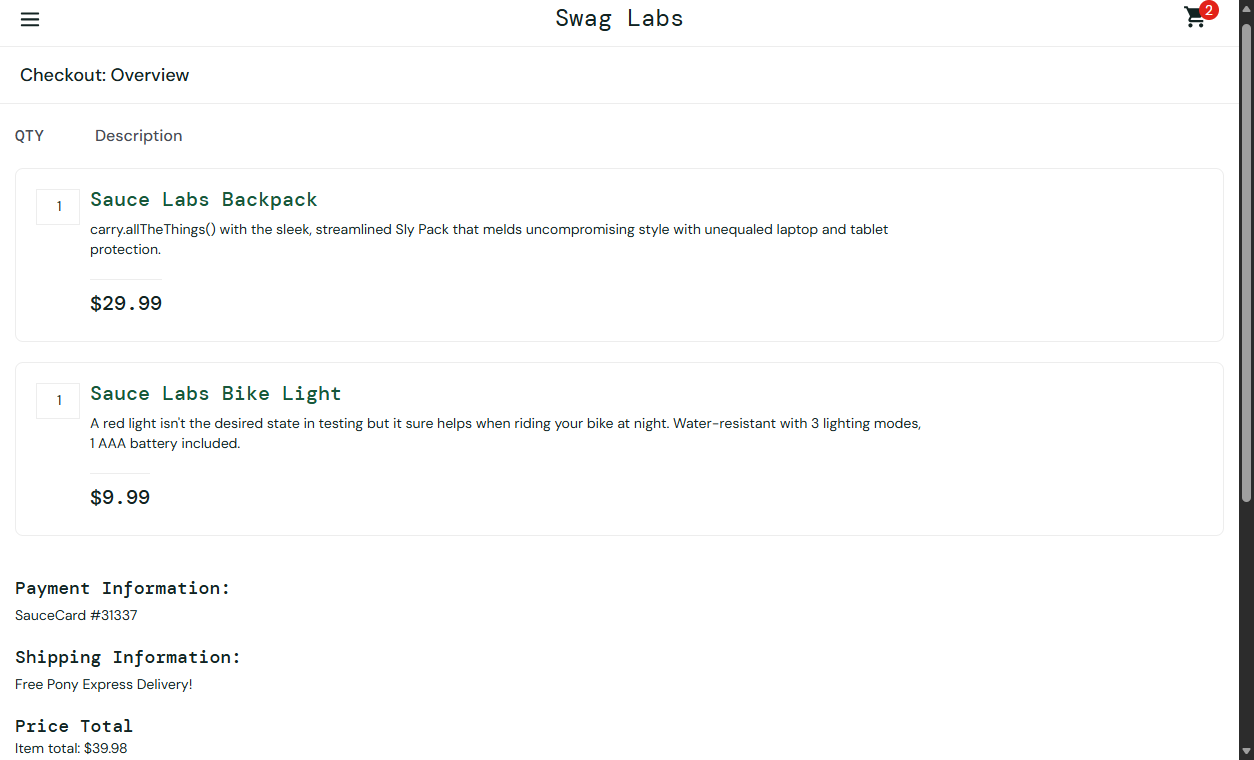
\includegraphics[width=\textwidth]{../screenshots/10_checkout_invalid_data_accepted.png}}
\caption{DEF-05 invalid data accepted}
\end{subfigure}
\hfill
\begin{subfigure}{0.48\textwidth}
\fbox{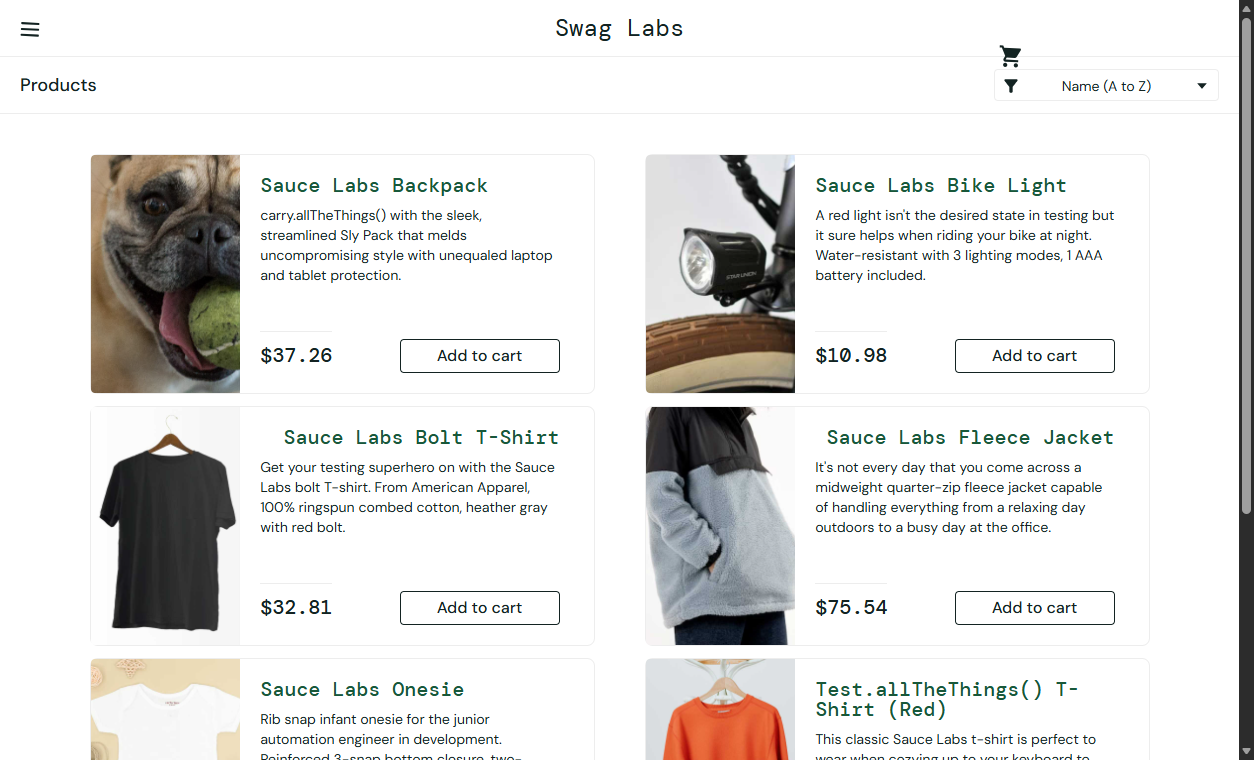
\includegraphics[width=\textwidth]{../screenshots/21_visual_user_layout.png}}
\caption{DEF-09 wrong prices, misaligned cart icon}
\end{subfigure}
\caption{Defect evidence}
\end{figure}

\section{Outputs}
\begin{itemize}
  \item \texttt{test\_cases/SwagLabs\_Test\_Cases.xlsx}: 39 test cases, 9 defects, RTM (6 requirements), summary.
  \item \texttt{docs/Test\_Plan.md}, \texttt{docs/Test\_Scenarios.md}, \texttt{docs/Test\_Cases.md}, \texttt{docs/Defect\_Reports.md}.
  \item \texttt{screenshots/}: 23 evidence images.
\end{itemize}
Summary sheet values: total 39, passed 28, failed 11, pass percentage 71.8\%, defects 9 (critical 1, high 3, medium 5, low 0).

% =====================================================================
\chapter{Deployment and Maintenance}
\section{Installation and un-installation}
No installation is required to use the test package: open the Excel workbook and the Markdown files. To regenerate them:
\begin{lstlisting}
git clone https://github.com/VishwajeetTulse/ecommerce-manual-testing
pip install openpyxl selenium
python tools/build_documents.py      # rebuild workbook and Markdown
python tools/capture_evidence.py     # re-capture screenshots (Edge/Chrome)
\end{lstlisting}
\section{User help}
To execute the suite: open \url{https://www.saucedemo.com}, take the Test Cases sheet, filter by Module, log in as the user named in Test Data (password \texttt{secret\_sauce}), follow the steps, compare with Expected Result, fill Actual Result and Status, and for every Fail add a screenshot and a row in the Defect Reports sheet. Use the side-menu ``Reset App State'' between cases that need an empty cart.

% =====================================================================
\chapter{Conclusion and Future Scope}
This mini project carried out the complete manual testing process on a real e-commerce website. Starting from a test plan and twenty scenarios, thirty-nine test cases were designed with black-box techniques and executed by hand with six test users. Eleven failures were traced to nine defects, documented with severity, priority, reproduction steps and screenshots, and a traceability matrix links every requirement to its tests. The work shows that systematic manual testing with well-chosen negative cases and special test users finds a wide range of functional, visual and performance defects.

Future scope: extend coverage to accessibility and cross-browser testing, add exploratory testing sessions with charters, convert the stable passing cases into automated regression scripts (done in the companion automation project), and track defects in a tool such as Jira with the life cycle shown in Fig.\ref{fig:state-dig}.

% =====================================================================
\begin{thebibliography}{99}
\bibitem{myers2011} G. J. Myers, C. Sandler and T. Badgett. 2011. \emph{The Art of Software Testing} (3rd ed.). John Wiley \& Sons.
\bibitem{jorgensen2013} P. C. Jorgensen. 2013. \emph{Software Testing: A Craftsman's Approach} (4th ed.). CRC Press.
\bibitem{kaner1999} C. Kaner, J. Falk and H. Q. Nguyen. 1999. \emph{Testing Computer Software} (2nd ed.). John Wiley \& Sons.
\bibitem{itkonen2007} J. Itkonen, M. V. M\"antyl\"a and C. Lassenius. 2007. Defect detection efficiency: test case based vs. exploratory testing. In \emph{Proc. First International Symposium on Empirical Software Engineering and Measurement (ESEM)}. IEEE, 61--70.
\bibitem{itkonen2009} J. Itkonen, M. V. M\"antyl\"a and C. Lassenius. 2009. How do testers do it? An exploratory study on manual testing practices. In \emph{Proc. ESEM 2009}. IEEE, 494--497.
\bibitem{bertolini2010} C. Bertolini and A. Mota. 2010. A framework for GUI testing based on use case design. In \emph{Proc. ICST Workshops}. IEEE, 252--259.
\bibitem{garousi2016} V. Garousi and M. V. M\"antyl\"a. 2016. When and what to automate in software testing? A multi-vocal literature review. \emph{Information and Software Technology} 76 (2016), 92--117.
\bibitem{ieee829} IEEE. 2008. \emph{IEEE Standard for Software and System Test Documentation} (IEEE Std 829-2008).
\bibitem{istqb} ISTQB. 2018. \emph{Certified Tester Foundation Level Syllabus}. International Software Testing Qualifications Board.
\bibitem{saucedemo} Sauce Labs. \emph{Swag Labs sample application}. \url{https://www.saucedemo.com}
\bibitem{bookPressman} R. S. Pressman. 2010. \emph{Software Engineering: A Practitioner's Approach} (7th ed.). McGraw-Hill.
\end{thebibliography}

% =====================================================================
\begin{appendices}

\chapter{Laboratory assignments on Project Analysis of Algorithmic Design}
\begin{itemize}
\item \textbf{IDEA Matrix.} Increase: defect detection. Drive: requirement coverage. Educate: testers on bug reporting. Accelerate: regression through reusable cases. Improve: input validation of the site. Deliver: Excel test package. Evaluate: pass percentage per module. Associate: failures with defects. Ignore: payment internals. Decrease: ambiguity in steps. Eliminate: unreproducible failures. Avoid: untraced cases.
\item \textbf{Feasibility.} Minimal test-suite selection is NP-hard in general (set cover), but with 6 requirements and 39 cases the RTM was completed by inspection. Execution cost is linear in the number of cases.
\item \textbf{Function.} $x$ = (test case, user), $y = f(x) \in \{\mathrm{Pass}, \mathrm{Fail}\}$ with $f(x) = \mathrm{Pass} \iff actual = expected$.
\end{itemize}

\chapter{Laboratory assignments on Project Quality and Reliability Testing of Project Design}
\begin{itemize}
\item \textbf{Objects and morphisms.} Objects: Requirement, Scenario, TestCase, Defect. Morphisms: expand (Scenario $\to$ TestCase), execute (TestCase $\to$ status), report (failed TestCase $\to$ Defect), trace (Requirement $\to$ TestCase).
\item \textbf{Functional dependency graph.} Defect depends on TestCase; TestCase depends on Scenario and Requirement; Summary depends on all TestCase statuses (see Fig.\ref{fig:dfd1}).
\item \textbf{Test data.} Equivalence classes: username $\in$ \{valid, empty, unknown, locked\}; password $\in$ \{correct, wrong, empty\}; first/last name $\in$ \{letters, digits, symbols, empty\}; postal code $\in$ \{digits, letters, empty\}.
\item \textbf{Black-box test cases.} 39 cases in the workbook; selection in Table \ref{tab:tests}.
\end{itemize}

\chapter{Project Planner}
\label{app:plan}
\begin{table}[H]
\begin{center}
\def\arraystretch{1.3}
\begin{tabularx}{\textwidth}{| c | X | c | c |}
\hline
Week & Activity & Deliverable & Status \\ \hline
1 & Study Swag Labs, list requirements, write test plan and scenarios & Test\_Plan.md, Test\_Scenarios.md & Done \\ \hline
2 & Design 39 test cases in Excel; guide review & SwagLabs\_Test\_Cases.xlsx & Done \\ \hline
3 & Execute with six users, capture evidence, log defects & Status column, screenshots, Defect sheet & Done \\ \hline
4 & RTM, summary, repository, report & RTM sheet, report.pdf & Done \\ \hline
\end{tabularx}
\end{center}
\caption{Project planner}
\end{table}

\chapter{Reviewers Comments of Paper Submitted}
Not applicable for this mini project.

\chapter{Plagiarism Report}
To be attached after checking through the institute's plagiarism tool.

\chapter{Term-II Project Laboratory Assignments}
\begin{enumerate}
\item Review of design: the guide's suggestion to use all six test users, not only \texttt{standard\_user}, was adopted and produced most of the defects.
\item Project workstation: Windows 11 laptop with Microsoft Edge 142, Excel, Python 3.14 and Git.
\item Execution: completed as described in Chapters 8 and 9.
\item Test results: 39 cases, 28 pass, 11 fail, 9 defects; module-wise chart in Table \ref{tab:summary}.
\end{enumerate}

\chapter{Information of Project Group Members}
\begin{enumerate}
\item Name : Vishwajeet Tulse
\item Date of Birth :
\item Gender :
\item Permanent Address :
\item E-Mail :
\item Mobile/Contact No. :
\item Placement Details :
\item Paper Published : --
\end{enumerate}
\newpage
\begin{enumerate}
\item Name : Student Name 2
\item Date of Birth :
\item Gender :
\item Permanent Address :
\item E-Mail :
\item Mobile/Contact No. :
\item Placement Details :
\item Paper Published : --
\end{enumerate}
\newpage
\begin{enumerate}
\item Name : Student Name 3
\item Date of Birth :
\item Gender :
\item Permanent Address :
\item E-Mail :
\item Mobile/Contact No. :
\item Placement Details :
\item Paper Published : --
\end{enumerate}
\newpage
\begin{enumerate}
\item Name : Student Name 4
\item Date of Birth :
\item Gender :
\item Permanent Address :
\item E-Mail :
\item Mobile/Contact No. :
\item Placement Details :
\item Paper Published : --
\end{enumerate}
\end{appendices}

\end{document}
